\chapter{Maß  und Integrationstheorie}
\label{\detokenize{masstheorie/intro_masstheorie:masz-und-integrationstheorie}}\label{\detokenize{masstheorie/intro_masstheorie::doc}}
\par
Im ersten Semester haben wir bereits das \emph{Riemann Integral} zur Berechnung des Flächeninhalts zwischen einer Funktion \(f \colon [a,b] \rightarrow \R\) und der x Achse eingeführt (siehe Kapitel 7 in \cite{Bur20}).
Die grundlegende Idee hierbei war es die x Achse in (unterschiedlich große) Intervalle zu unterteilen und mittels dieser Zerlegung Rechtecke zwischen dem Graphen der Funktion und der x Achse zu konstruieren.
Durch das Produkt der Seitenlängen dieser Rechtecke lässt sich nämlich deren Flächeninhalt leicht berechnen und die Summe all dieser Flächeninhalte approximiert den wahren Flächeninhalt zwischen dem Graphen und \(f\) und der x Achse.
Dieses Vorgehen ist zur Erinnerung nochmal in Abbildung \hyperref[\detokenize{masstheorie/intro_masstheorie:fig-riemann-integral}]{Abb.\@ \ref{\detokenize{masstheorie/intro_masstheorie:fig-riemann-integral}}} illustriert.

\begin{figure}[htbp]
\centering


\noindent\includegraphics[width=\textwidth]{../\string_build/html/\string_images/ober\string_untersummen.png}
\caption{Illustration zweier Approximationen des Riemann Integrals einer Funktion durch den Flächeninhalt von Rechtecken. Die grünen und lila Rechtecke visualisieren die Unter  bzw. Obersummen bezüglich des in rot dargestellten Graphen der Funktion. Quelle: \href{https://de.wikipedia.org/wiki/Riemannsches\_Integral}{Wikipedia; Riemannsches Integral}.}\label{\detokenize{masstheorie/intro_masstheorie:fig-riemann-integral}}\end{figure}

\par
Da wir bisher nur die Integration von eindimensionalen Funktionen auf kompakten Intervallen kennengelernt haben, wollen wir in diesem Kapitel den Begriff des Integals auf mehrdimensionale Funktionen \(f \colon \R^n \rightarrow \R\) erweitern.
Das Riemann Integral lässt sich problemlos auf mehrdimensionalen Funktionen verallgemeinern, indem man das Integral nicht durch den Flächeninhalt von Rechtecken approximiert, sondern hierfür das \emph{Volumen von entsprechenden Quadern} \(Q \subset \R^n\) berechnet.
Es lässt sich insbesondere zeigen, dass jede stetige mehrdimensionale Funktion auf einem (nicht ausgeartetem) Quader Riemann integrierbar ist.

\par
Es hat sich jedoch in der Entwicklung der Mathematik herausgestellt, dass der Begriff des Riemann Integrals zu starke Forderungen an die zu Grunde liegenden Funktionen stellt und damit wichtige und interessante Funktionsklassen nicht integrierbar waren.
Als Beispiel hierfür seien \href{https://de.wikipedia.org/wiki/Fraktal}{fraktale Mengen und Funktionen} genannt, welche auch zur Modellierung von Prozessen in der Natur genutzt werden.

\par
Aus diesem Grund hat sich ein eigenes Feld innerhalb der modernen Analysis gebildet   die sogenannte \textbf{Maßtheorie}.
Es widmet sich hauptsächlich der Untersuchung von Maßen zur Berechnung von Längen, Flächen und Volumina in unterschiedlichen mathematischen Strukturen und Räumen.
Es wird klar, dass Integration und die Berechnung von Volumina eng miteinander zusammen hängen, denn ist \(A\subset\R^n\) eine (messbare) Teilmenge, dann ist ihr Maß gleich dem Integral ihrer charakteristischen Funktion, d.h.,
\begin{align*}
\int_{\R^n} \mathbb{1}_A(x)\,\mathrm{d}x.
\end{align*}
\par
In einem gewissen Sinn sind Maße ein \emph{fundamentaleres Konzept} als das der Integration, da sich jede Integration auf die Berechnung von Maßen stützt.

\par
Eins der berühmtesten Beispiele zur Motivation der Maßtheorie ist im Folgenden erklärt.
\begin{example}{(Dirichlet Funktion)}{masstheorie/intro_masstheorie:ex:dirichletFunktion}



\par
Wir betrachten das kompakte Intervall \([0,1] \subset \R\) und definieren hierauf die sogenannte \textbf{Dirichlet Funktion} \(\mathbb{1}_\Q \colon [0,1] \rightarrow \{0,1\}\) mit
\begin{align*}
\mathbb{1}_\Q(x) := \begin{cases} 1, \ \text{ falls } x \in \Q, \\ 0, \ \text{ sonst }.\end{cases}
\end{align*}
\par
Diese Abbildung kann als \emph{charakteristische Funktion} der rationalen Zahlen \(\Q\) aufgefasst werden.
Man sieht leicht ein, dass diese Funktion \textbf{nicht Riemann integrierbar} ist, da alle Untersummen stets \(0\) und alle Obersummen stets \(1\) sind.
\end{example}

\par
Um eine Funktion wie die Dirichlet Funktion in \cref{masstheorie/intro_masstheorie:ex:dirichletFunktion} zu integrieren sieht man zunächst ein, dass die rationalen Zahlen \(\Q\) in den reellen Zahlen \(\R\) als abzählbare Menge eine sogenannte \emph{Nullmenge} im Sinne der Maßtheorie repräsentieren.
Wir werden im Laufe der Vorlesung die nötigen Werkzeuge der Maßtheorie einführen um diesen Umstand zu verstehen und einen verallgemeinerten Begriff des Integrals definieren, der diese Nullmenge berücksichtigt   das \textbf{Lebesgue Integral}.
Dieses Integral ist eine echte Verallgemeinerung des Riemann Integrals und wir werden einsehen, dass die Menge der Lebesgue integrierbaren Funktionen eine Obermenge der Menge der Riemann integrierbaren Funktionen ist.
Außerdem verhält sich das Lebesgue Integral bei Grenzwertbildungen einfacher als das Riemann Integral.


\section{Maßtheorie}
\label{\detokenize{masstheorie/masstheorie:masztheorie}}\label{\detokenize{masstheorie/masstheorie::doc}}
\par
Wir wollen in diesem Kapitel formal die Maßtheorie einführen, die es uns erlaubt zu entscheiden welche Mengen messbar sind und wie sich das Volumen von Mengen in topologischen Räumen bestimmen lässt.
Die hier beschriebenen Werkzeuge werden uns im nächsten Kapitel bei der Einführung des \emph{Lebesgue Integrals} als Verallgemeinerung des Riemann Integrals sehr dienlich sein.

\par
Intuitiv ordnet ein \href{https://de.wikipedia.org/wiki/Ma\%c3\%9f\_(Mathematik)}{\textbf{Maß}} \(\mu\), welches auf einer Menge \(\Omega\) definiert ist, wie z.B. dem \(\R^n\), allen geeigneten Teilmengen \(A\subseteq \Omega\) nichtnegative reelle Zahlen zu, d.h.
\begin{align*}
\mu(A)\in[0,\infty] := [0,\infty)\cup\{\infty\}.
\end{align*}
\par
Hierbei soll das Maß \(\mu\) natürlich mit dem Volumen der Teilmenge \(A\) zusammenhängen.
Man beachte, dass wir auch explizit unendliche Maße zulassen, z.B., falls die Menge \(\Omega\) schon der gesamte \(\R^n\) ist.

\par
Bevor wir den Begriff des Maßes formal definieren können und dessen Eigenschaften näher diskutieren, müssen wir jedoch noch mehr Verständnis für die zu Grunde liegenden Mengen und Mengensystem entwickeln.


\subsection{\protect\(\sigma\protect\) Algebren und Maße}
\label{\detokenize{masstheorie/masstheorie:sigma-algebren-und-masze}}\label{\detokenize{masstheorie/masstheorie:s-sigmaalg}}
\par
Wir betrachten im Folgenden eine beliebige zu Grundmenge \(\Omega\), welche endlich, abzählbar oder auch überabzählbar sein kann. Ein Maß soll nun Teilmengen von \(\Omega\) einen Wert zuordnen weshalb wir die \textbf{Potenzmenge} \(2^\Omega\) betrachten, welche die Menge aller möglichen Teilmengen von \(\Omega\) bildet. Ein Maß ist dann (unter zusätzlichen Voraussetzungen, siehe \cref{masstheorie/masstheorie:def:mass}  eine spezielle Abbildung \(\mu:\Sigma\to[0,\infty]\), wobei \(\Sigma\subset 2^\Omega\) ein Mengensystem ist, welches man auch System der \(\mu\) messbaren Mengen nennt.

\begin{emphBox}{}{}{Bemerkung:}
\par
Mengen von Mengen nennen wir häufig auch \emph{Mengensysteme}.
\end{emphBox}

\par
Bei der Konstruktion eines Maßes gibt es zwei teilweise konkurrierende Wünsche:
\begin{enumerate}

\item {} 
\par
Möglichst vielen Mengen soll ein Volumen zugeordnet werden können, d.h., \(\Sigma\) soll groß sein.

\item {} 
\par
Das Maß disjunkt vereinigter Mengen soll gleich der Summe der einzelnen Maße sein.

\end{enumerate}

\par
Der erste Wunsch würde darauf hindeuten die Potenzmenge \(2^\Omega\) als System der messbaren Mengen zu betrachten. Allerdings gibt es viele Fälle (siehe \cref{masstheorie/masstheorie:s-vitali} ) in welchen diese Wahl den zweiten Wunsch unmöglich machen. Deshalb ist die Strategie meist ein möglichst großes Teilmengensystem zu finden, s.d. der zweite Wunsch erfüllbar ist. Die Klasse von Systemen auf der wir im Folgenden arbeiten werden, sind sogenannte \(\sigma\) Algebren.
\begin{definition}{(\protect\(\sigma\protect\) Algebra und Messraum)}{masstheorie/masstheorie:def:sigmaalgebra}



\par
Ein Mengensystem \(\Sigma \subseteq 2^\Omega\) heißt \textbf{\(\sigma\) Algebra (von \(\Omega\))}, wenn die folgenden Eigenschaften erfüllt sind
\begin{enumerate}

\item {} 
\par
\(\Omega\in \Sigma\)

\item {} 
\par
\(A\in \Sigma \quad \Rightarrow \quad A^c:=\Omega \setminus A\in \Sigma\)

\item {} 
\par
\((A_n)_{n\in\N} \in \Sigma \quad \Rightarrow \quad \bigcup_{n\in \N} A_n\in \Sigma\).

\end{enumerate}

\par
Für eine \(\sigma\) Algebra \(\Sigma \subseteq \mathcal{P}(\Omega)\) von \(\Omega\) nennen wir das Paar (\(\Omega,\Sigma\)) \textbf{Messraum} und die Mengen des Mengensystems \(\Sigma\) heißen \textbf{messbar}.
\end{definition}

\par
Das Symbol \(\sigma\) erinnert an den Begriff der Summe, insbesondere wegen der dritten Eigenschaft in \cref{masstheorie/masstheorie:def:sigmaalgebra}  also der Abgeschlossenheit unter abzählbarer Vereinigung von Teilmengen.
Aus diesen drei Eigenschaften lässt sich auch direkt zeigen, dass \(\sigma\) Algebren ebenfalls unter \emph{abzählbaren Schnitten} abgeschlossen sind, wie das folgende Lemma zeigt.
\begin{lemma}{(Abgeschlossenheit unter abzählbaren Schnitten)}{masstheorie/masstheorie:lemma-1}



\par
Es sei (\(\Omega,\Sigma\)) ein Messraum und es sei \((A_i)_{i\in_\N}\) eine Familie von Elementen der \(\sigma\) Algebra \(\Sigma\) mit \(A_i \in \Sigma\) für \(i \in \N\).
Dann sind abzählbare Schnitte dieser Mengen auch Elemente der \(\sigma\) Algebra \(\Sigma\), d.h.,
\begin{align*}
\bigcap_{n \in \N} A_n \in \Sigma.
\end{align*}\end{lemma}

\begin{proof}
 Es reicht die Aussage für \(n=2\) zu zeigen. Seien dazu \(A_1,A_2\in\Sigma\), dann folgt \(A_1^C,A_2^C\in\Sigma\) und somit auch \(A^C\cup A_2^C\in\Sigma\). Und somit folgt
\begin{align*}
A_1\cap A_2 = (A_1^C\cup A_2^C)^C \in \Sigma.
\end{align*}\end{proof}

\par
Aus der \cref{masstheorie/masstheorie:def:sigmaalgebra} kann man sich leicht zwei Spezialfälle von \(\sigma\) Algebren überlegen.
Es wird klar, dass das Mengensystem \(\{\emptyset, \Omega\}\) die kleinstmögliche \(\sigma\) Algebra bildet, wohingegen die Potenzmenge \(\mathcal{P}(\Omega)\) die größtmögliche \(\sigma\) Algebra darstellt.

\par
Für ein beliebiges Mengensystem \(\mathcal{C}\subset 2^\Omega\) können wir zusätzlich die erzeugt \(\sigma\) Algebra betrachten, welche die kleinste \(\sigma\) Algebra ist die \(\mathcal{C}\) enthält.
\begin{definition}{(Erzeugte \protect\(\sigma\protect\) Algebra)}{masstheorie/masstheorie:definition-2}



\par
Es sei \(\mathcal{C}\subset 2^\Omega\) ein Mengensystem, dann bezeichnen wir mit
\begin{align*}
\sigma(\mathcal{C}) := \bigcup_{\substack{\Sigma \text{ ist $\sigma$-Algebra}\\ \mathcal{C} \subset \Sigma}} \Sigma
\end{align*}
\par
die von \(\mathcal{C}\) erzeugte \(\sigma\) Algebra.
\end{definition}

\par
Für die erzeugt \(\sigma\) Algebra, haben wir folgende Eigenschaften.
\begin{lemma}{}{masstheorie/masstheorie:lemma-3}



\par
Es sei \(\mathcal{C}\subset 2^\Omega\) ein Mengensystem, dann gilt
\begin{enumerate}

\item {} 
\par
\(\sigma(\mathcal{C})\) ist eine \(\sigma\) Algebra.

\item {} 
\par
\(\sigma(\mathcal{C})\) ist die kleinste \(\sigma\) Algebra die \(\mathcal{C}\) enthält, d.h., falls \(\mathcal{C}\subset\Sigma\) eine weitere \(\sigma\) Algebra ist, so folgt \(\sigma(\mathcal{C})\subset\Sigma\).

\item {} 
\par
Falls \(\mathcal{C}\) selbst eine \(\sigma\) Algebra ist, so folgt \(\sigma(\mathcal{C}) = \mathcal{C}\).

\end{enumerate}
\end{lemma}

\begin{proof}
 Übung.
\end{proof}


\subsection{Maße}
\label{\detokenize{masstheorie/masstheorie:masze}}
\par
Basierend auf dem Begriff einer \(\sigma\) Algebra und eines Messraums können wir nun formal einführen, was wir unter einem Maß verstehen.
\begin{definition}{(Maß und Maßraum)}{masstheorie/masstheorie:def:mass}



\par
Sei \((\Omega, \Sigma)\) ein Messraum.
Wir nennen eine Abbildung \(\mu: \Sigma\to [0, \infty]\) \textbf{Maß}, wenn die folgenden beiden Eigenschaften erfüllt sind.
\begin{enumerate}

\item {} 
\par
Die leere Menge hat das Maß Null, d.h., \(\mu(\emptyset) = 0\),

\item {} 
\par
Für eine Familie von disjunkten Mengen \((A_n)_{n\in\N}\) der \(\sigma\) Algebra \(\Sigma\) mit \(A_i \cap A_j = \emptyset\) für \(i \neq j\) gilt die sogenannte abzählbare oder \(\sigma\) \textbf{Additivität}, d.h.,

\end{enumerate}
\begin{align*}
\mu\left( \bigcup_{n\in\N}A_n \right) = \sum_{n\in\N}\mu (A_n).
\end{align*}
\par
Wir nennen das Maß \(\mu\) \textbf{endlich}, wenn \(\mu(\Omega)<\infty\).
Das Tripel \((\Omega, \Sigma, \mu)\) wird als \textbf{Maßraum} bezeichnet.
\end{definition}
\begin{remark}{}{masstheorie/masstheorie:rem:wahrscheinlichkeitsmass}



\par
Maße spielen insbesondere in der \emph{Wahrscheinlichkeitstheorie} eine zentrale Rolle, um die Wahrscheinlichkeit von Ereignismengen anzugeben.
Dabei wird nicht nur gefordert, dass das Maß \(\mu\) endlich sein muss, sondern dass sogar \(\mu(\Omega)=1\) gilt, damit es sich um ein \textbf{Wahrscheinlichkeitsmaß} handelt.
Diese finden vor allem in der Quantenmechanik Anwendung.
\end{remark}

\par
Aus den beiden grundlegenden Eigenschaften eines Maßes lassen sich weitere nützliche Eigenschaften herleiten, wie das folgende Lemma beschreibt.
\begin{lemma}{(Eigenschaften von Maßen)}{masstheorie/masstheorie:lemma-6}



\par
Sei \((\Omega, \Sigma, \mu)\) ein Maßraum.
Dann gelten die folgenden Eigenschaften für das Maß \(\mu \colon \Sigma \rightarrow [0,\infty]\).

\par
1. Für \(A,B \in \Sigma\) mit \(B \subset A\) und \(\mu(B) < \infty\) gilt:
\begin{align*}
\mu(A \setminus B) = \mu(A) - \mu(B) \qquad \text{(Subtraktivität)}
\end{align*}
\par
2. Für \(A,B \in \Sigma\) mit \(B \subset A\) gilt:
\begin{align*}
\mu(B) \leq \mu(A) \qquad \text{(Monotonie)}
\end{align*}
\par
3. Für \(A,B \in \Sigma\) gilt stets:
\begin{align*}
\mu(A \cup B) = \mu(A) + \mu(B) - \mu(A \cap B).
\end{align*}\end{lemma}

\begin{proof}
 In der Hausaufgabe zu zeigen.
\end{proof}

\par
Im Folgenden wollen wir ein paar Beispiele von geläufigen Maßen diskutieren.
\begin{example}{(Maße)}{masstheorie/masstheorie:example-7}



\par
Wichtige Maße in der Mathematik und Physik sind beispielsweise die folgenden.

\par
1. Das \href{https://de.wikipedia.org/wiki/Z\%c3\%a4hlma\%c3\%9f\_(Ma\%c3\%9ftheorie)}{\textbf{Zählmaß}} \(m\) auf einer \emph{endlichen} Menge \(M\), mit
\begin{align*}
m(A):=|A|\qquad (A\subseteq M).
\end{align*}
\par
Hier sind insbesondere alle Teilmengen messbar, d.h., \((M, \mathcal{P}(M), m)\) bildet einen Maßraum.

\par
2. Das \textbf{Lebesgue–Maß} \(\lambda^n\) auf dem \(\R^n\), das wir bald kennen lernen, zeichnet sich dadurch aus, dass es einer verschobenen Menge das gleiche Volumen zuordnet wie einer unverschobenen.
Es besitzt also die nützliche Eigenschaft \emph{translations } und \emph{rotationsinvariant} zu sein.
Dies gilt ebenfalls für Spiegelungen.
Außerdem ordnet das Lebesgue Maß dem Einheitswürfel \([0,1]^n\) das Maß \(1\) zu, was unserer Intuition entspricht.
Andererseits stellt sich heraus, dass das Lebesgue Maß nicht auf der gesamten Potenzmenge \(\mathcal{P}(\R^n)\) definiert werden kann.

\par
3. Das \href{https://de.wikipedia.org/wiki/Diracma\%c3\%9f}{\textbf{Dirac Maß}} \(\delta_x\) ist im Punkt \(x \in \R^n\) konzentriert, und für jede Teilmenge \(A\subset\R^n\) gilt
\begin{align*}
\delta_x(A) \equiv \int_A\delta_x := \begin{cases} 1, &  \text{ falls } x \in A,\\ 0, & \text{ sonst}. \end{cases}
\end{align*}
\par
Dieses Maß ist im Gegensatz zum Lebesgue Maß nicht translationsinvariant, da es explizit von der Lage des Punkts \(x\in\R^n\) abhängt.
Es wird beispielsweise in der Elektrodynamik benutzt, um eine in \(x\) lokalisierte, punktförmige Ladung zu beschreiben.

\par
4. Häufig möchte man die Länge einer \emph{Kurve} oder allgemeiner den Flächeninhalt einer \(d\) dimensionalen Fläche im \(\R^n\) messen.
Auch das dafür benutzte Maß \(\mu_d\) ist translations  und rotationsinvariant, es ordnet aber der \(d\) dimensionalen Einheitsfläche \([0,1]^d\times\{0\} \subset\R^d\times\R^{n-d}=\R^n\) das Maß \(1\) zu.
Entsprechend hat aber für \(d<n\) der Einheitswürfel das Maß \(\mu_d([0,1]^n)=\infty\).

\par
5. Man kann sogar sogenannte \href{https://de.wikipedia.org/wiki/Hausdorff-Ma\%c3\%9f}{\textbf{Hausdorff Maße}} \(\mu_d\) konstruieren, die Mengen beliebiger fraktaler Dimension \(d\in[0,n]\) messen.
Genau genommen \emph{definiert} man hierbei die Dimension der Menge \(A\subset \R^n\) durch \(d(A):=\inf\{d'>0\mid \mu_{d'}(A)=0\}.\)

\par
6. Im Zusammenhang mit dem sogenannten Feynmanschen \href{https://de.wikipedia.org/wiki/Pfadintegral}{\textbf{Pfadintegral}} der Quantenmechanik wird auf dem unendlich dimensionalen Raum \(\Omega\) der Weg zwischen zwei Punkten des Konfigurationsraumes \(\R^d\) ein \emph{Wahrscheinlichkeitsmaß} (siehe \cref{masstheorie/masstheorie:rem:wahrscheinlichkeitsmass}  definiert.
Dabei erhalten Pfade, die in der Nähe von Lösungskurven der DGL der Klassischen Mechanik sind, ein größeres Gewicht als beliebige Pfade.
\end{example}

\par
Eine sehr nützliche Eigenschaft von gewissen Maßen auf topologischen Räumen ist die der Regularität, welche wir im Folgenden definieren wollen.
\begin{definition}{(Regularität von Maßen)}{masstheorie/masstheorie:def:regularitaet}



\par
Es sei \((\Omega, \tau)\) ein topologischer Raum und \((\Omega, \Sigma, \mu)\) ein entsprechender Maßraum auf \(\Omega\), so dass gilt \(\tau \subset \Sigma\).
Dann können wir die Regulariät des Maßes \(\mu\) wie folgt definieren.
\begin{enumerate}

\item {} 
\par
Wir nennen das Maß \(\mu\) von \textbf{außen regulär}, wenn zu jeder messbaren Menge \(A \in \Sigma\) und jedem \(\epsilon > 0\) eine offene Obermenge \(U \in \tau\) existiert mit \(A \subset U\), so dass für das Maß \(\mu(U\setminus A) < \epsilon\) gilt.

\item {} 
\par
Wir nennen das Maß \(\mu\) von \textbf{innen regulär}, wenn zu jeder messbaren Menge \(A \in \Sigma\) und jedem \(\epsilon > 0\) eine abgeschlossene Teilmenge \(F \subset A\) gibt, so dass für das Maß \(\mu(A\setminus F) < \epsilon\) gilt.

\end{enumerate}
\end{definition}


\subsection{Borel Maße}
\label{\detokenize{masstheorie/masstheorie:borel-masze}}
\par
Neben \(\sigma\) Algebren kennen wir auch Topologien als wichtige Klasse von Mengensystemen, da diese es z.B. erlauben Stetigkeit von Funktionen zu definieren. Wir betrachten nun ein Konzept welches den Begriff einer Topologie mit der einer \(\sigma\) Algebra vereint, die sogenannte \textbf{Borel} \(\sigma\) Algebra.

\begin{emphBox}{}{}

\par
\href{https://de.wikipedia.org/wiki/\%C3\%89mile\_Borel}{Émile Borel} (geboren am 7. Januar 1871 in Saint Affrique; gestorben am 3. Februar 1956 in Paris) war ein französischer Mathematiker und Politiker.
\end{emphBox}
\begin{definition}{(Borel \protect\(\sigma\protect\) Algebra)}{masstheorie/masstheorie:definition-9}



\par
Die \textbf{Borel \(\sigma\) Algebra} auf einem topologischen Raum \((\Omega, \tau)\) ist die von \(\tau\) erzeugte \(\sigma\) Algebra,
\begin{align*}
\B(\Omega) := \sigma(\tau).
\end{align*}\end{definition}
\begin{remark}{(Borelsche \protect\(\sigma\protect\) Algebra von \protect\(\R\protect\))}{masstheorie/masstheorie:remark-10}



\par
Wir bemerken, dass die Borelsche \(\sigma\) Algebra von \(\R\) \textbf{nicht} alle Teilmengen von \(\R\) enthält.
Es lässt sich sogar zeigen, dass die borelsche \(\sigma\) Algebra von \(\R\) gleichmächtig zu \(\R\) ist, während die Potenzmenge \(2^\R\) eine echt größere Mächtigkeit als \(\R\) besitzt.
\end{remark}

\par
Man erkennt an der Notaion, dass die Topologie \(\tau\) meist unterschlagen wird. Man spricht meist auch vom topologischen Raum \(\Omega\) ohne \(\tau\) zu nennen.
Ein Maß auf dieser \(\sigma\) Algebra nennen wir auch \textbf{Borel Maß}.
\begin{definition}{}{masstheorie/masstheorie:definition-11}



\par
Es sei \(\Omega\) ein topologischer Raum, dann heißt ein Maß \(\mu\) auf \(\B(\Omega)\) Borel Maß.
\end{definition}


\subsubsection{Erzeugte Topologien}
\label{\detokenize{masstheorie/masstheorie:erzeugte-topologien}}\label{\detokenize{masstheorie/masstheorie:s-gentop}}
\par
Das Konzept der erzeugten \(\sigma\) Algebra lässt sich auch auf Topologien übertragen. Hierbei betrachtet man meist eine sogenannte Basis einer Topologie.
\begin{definition}{}{masstheorie/masstheorie:definition-12}



\par
Es sei \((\Omega,\tau)\) ein topologischer Raum, ein System \(\mathcal{C}\subset 2^\Omega\) heißt Basis für \(\tau\), falls für jede Menge \(U\in\tau\) Teilmengen aus \(\mathcal{C}\) existieren, \(J\subset\mathcal{C}\), s.d.,
\begin{align*}
\bigcup_{A\in J} A = U.
\end{align*}
\par
In diesem Fall schreiben wir auch \(\tau(\mathcal{C})=\tau\).
\end{definition}

\par
Besonders relevant sind für uns die Mengensysteme, welche die kanonische Topologie für \(\R\) erzeugt. Hierbei wissen wir, dass alle offene \emph{Intervalle} der Form \((a,b)\subset \R\), sowie alle Intervalle der Form \((-\infty, b)\) und \((a, \infty)\) die euklidische Topologie in \(\R\) erzeugen. Wir betrachten weiterhin ein derartiges Mengenssystem bestehend aus Intervallen, welche die Borel \(\sigma\) Algebra erzeugt.
\begin{lemma}{}{masstheorie/masstheorie:lem:genborel}



\par
Es sei
\begin{align*}
\mathcal{C} = \{ [-\infty, c):c\in\R\}
\end{align*}
\par
dann gilt \(\sigma(\mathcal{C}) = \B(\overline{\R})\).
\end{lemma}


\subsubsection{Eigenschaften von Borel Maßen}
\label{\detokenize{masstheorie/masstheorie:eigenschaften-von-borel-maszen}}
\par
Für spezielle topologische Räume lässt sich eine wichtige Eigenschaft von Maßen über die Borel \(\sigma\) Algebra definieren.
\begin{definition}{(Lokale Endlichkeit von Maßen)}{masstheorie/masstheorie:definition-14}



\par
Sei \((\Omega, \tau)\) ein Haussdorf Raum (siehe \cref{manifolds/manifolds_prelim:def:hausdorffraum}  und sei \(\B(\Omega) = \sigma(\tau)\) die Borel \(\sigma\) Algebra, die durch \(\tau\) erzeugt wird.
Wir nennen ein Maß \(\sigma \colon \B(\Omega) \rightarrow [0, \infty]\) \textbf{lokal endlich}, falls jeder Punkt \(x \in \Omega\) eine lokale Umgebung mit endlichem Maß besitzt.
\end{definition}

\par
Die lokale Endlichkeit ist essentiell bei der Untersuchung von Maßen auf topologischen Räumen, weil sie für jeden Punkt die Existenz einer Umgebung mit endlichem Maß garantiert.
Wie wir später sehen werden ist das Lebesgue Maß auf dem Raum \(\R^n\) lokal endlich.

\par
Basierend auf der oben definierten Borel \(\sigma\) Algebra lässt sich nun das sogenannte Borel Maß einführen.
\begin{definition}{(Borel Maß)}{masstheorie/masstheorie:definition-15}



\par
Ein lokal endliches Maß \(\sigma \colon \B(\Omega) \rightarrow [0, \infty]\) auf der Borelschen \(\sigma\) Algebra eines Hausdorff Raums \((\Omega,\tau)\) heißt \textbf{Borel Maß}.
\end{definition}


\subsection{Das Lebesgue Maß}
\label{\detokenize{masstheorie/masstheorie:das-lebesgue-masz}}\label{\detokenize{masstheorie/masstheorie:s-lebesguemeasure}}
\begin{emphBox}{Henri Lebesgue}{}

\par
\href{https://en.wikipedia.org/wiki/Henri\_Lebesgue}{Henri Léon Lebesgue} (Geboren 28. Juni 1875 in Beauvais; Gestorben 26. Juli 1941 in Paris) war ein französischer Mathematiker.
\end{emphBox}

\par
Bei der Einführung des Riemann Integrals verwendet man Intervalle zur Unterteilung des Definitionsbereichs.
Diese Partitionierung einer Menge lässt sich im \(\R^n\) auf mehrdimensionale Quader verallgemeinern. Für \(a = (a_1,\ldots,a_n) \in \R^n\) und \(b = (b_1,\ldots,b_n) \in \R^n\) verwenden wir hierbei die Anordnungsrelation
\begin{align*}
a < b \qquad \Leftrightarrow \qquad a_i < b_i \quad i=1,\ldots,n
\end{align*}
\par
und analog für \(a \leq b, a > b\) und \(a \geq b\).
\begin{definition}{}{masstheorie/masstheorie:def:quader}



\par
und darüber im Folgenden \textbf{offene, halboffene} und \textbf{abgeschlossene Quader} im \(\R^n\) respektive beschreiben durch
\begin{align*}
(a,b) &= \lbrace x \in \R^n : a < x < b \rbrace,\\
(a,b] &= \lbrace x \in \R^n : a < x \leq b \rbrace,\\
[a,b] &= \lbrace x \in \R^n : a \leq x \leq b \rbrace.
\end{align*}
\par
Das \textbf{Volumen} bzw. der Lebesgue Inhalt eines halboffenen Quaders \(Q := (a,b] \subset \R^n\) definieren wir über
\begin{align*}
\lambda^n(Q) := \prod_{i=1}^n (b_i - a_i).
\end{align*}\end{definition}

\par
Wir wollen im Folgenden das Teilmengensystem \(\mathcal{R}_{\text{Q}}\subset\ 2^{\R^n}\) aller halboffenen Quader betrachten,
\begin{align*}
\mathcal{R}_{\text{Q}} := \left\{ \bigsqcup_{i=1,\ldots,k} Q_i \colon Q_i \text{ ist halboffener Quader im } \R^n \right\}.
\end{align*}
\par
Wir fordern hierbei nicht, dass nur disjunkte Quader vereinigt werden dürfen. Jedoch kann man direkt herleiten, dass man jede Vereinigung von Quadern in eine disjunkte Umschreiben kann. Seien dazu \(Q_1,\ldots,Q_k\subset\R^n\) halboffene Quader, wir erkennen, dass der Rand eines Quaders \(Q_i=(a^i,b^i]\) genau \(2n\) Hyperebenen der Form
\begin{align*}
x_j = a^i_j\\
x_j = b^i_j
\end{align*}
\par
für \(j=1,\ldots,n\) aufspannt. Weiterhin, können wir einen anderen Quader \(Q_m=(a^k,b^k)\) mit einer Hyperebene \(x_l=c\in\R\) zerteilen, im Falle \(a^k_l < c < b^k_l\), indem wir zwei neue Quader definieren mit
\begin{align*}
\alpha^m&:=(a^m_1,\ldots,c,\ldots,a^m_n)\\
\beta^m&:=(b^m_1,\ldots,c,\ldots,b^m_n)\\
Q_m^1&=(a^m,\beta^m]\\
Q_m^2&=(\alpha^m,b^m].
\end{align*}
\par
Iterativ gehen wir folgendermaßen vor:
\begin{enumerate}

\item {} 
\par
Betrachte den ersten Quader \(Q_1\), zerteile alle Quader \(Q_i\) an allen seinen Hyperebenen und erhalte so neue Quader \(W^1_j\).

\item {} 
\par
Im \(i+1\)ten Schritt betrachte die Hyperebenen des Quaders \(Q_{i+1}\) und zerteile damit alle Quader \(W^i_j\) aus dem vorherigen Schritt und erhalte damit neue Quader \(W^{i+1}_j\).

\end{enumerate}

\par
Führen wir diesen Prozess bis \(i=k\) durch, so erhalten wir folgendes Resultat, welches in \hyperref[\detokenize{masstheorie/masstheorie:fig-disrect}]{Abb.\@ \ref{\detokenize{masstheorie/masstheorie:fig-disrect}}} visualisiert ist.

\begin{figure}[htbp]
\centering


\noindent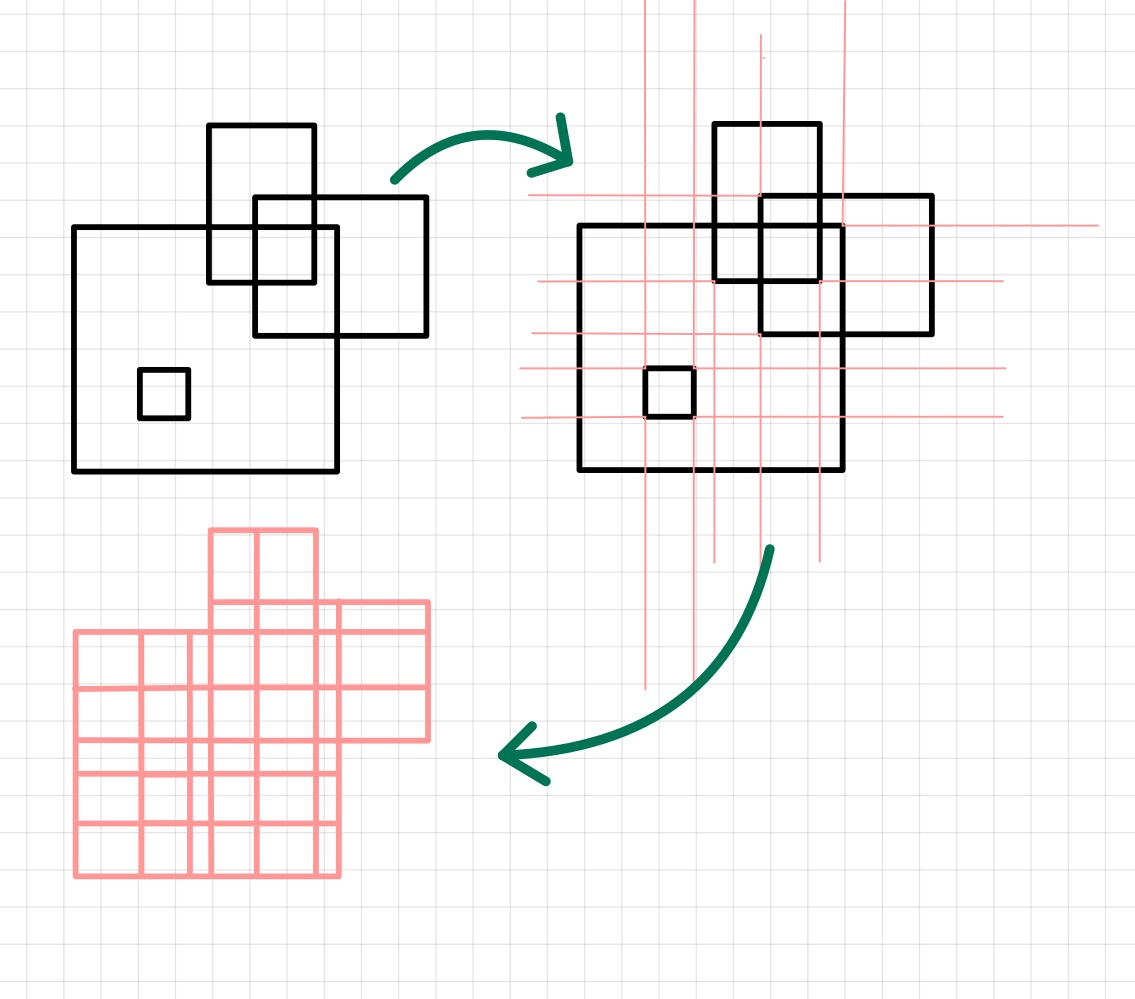
\includegraphics[width=\textwidth]{../\string_build/html/\string_images/DisRect.jpg}
\caption{Nicht disjunkte Quader werden in System disjunkter Quader überführt. Man erkennt insbesondere, dass die Vereinigung gleich bleibt und, dass sich jeder einzelne ursprüngliche Quader, aus den neuen Quadern zusammensetzbar ist.}\label{\detokenize{masstheorie/masstheorie:fig-disrect}}\end{figure}
\begin{lemma}{}{masstheorie/masstheorie:lem:disRect}



\par
Es seien \(Q_1,\ldots,Q_k\subset\R^d\) halboffene Quader, dann existieren paarweise disjunkte halboffene Quader \(W_1,\ldots, W_M\) mit Indexmengen \(J_i\subset\{1,\ldots,M\}\), s.d.
\begin{align*}
\bigcup_{i=1}^k Q_i = \bigcup_{j=^1}^M W_j
\end{align*}
\par
und für jedes \(i\in\{1,\ldots,n\}\) gilt
\begin{align*}
\bigcup_{j\in J_i} W_j = Q_i.
\end{align*}\end{lemma}

\par
Das System der halboffenen Quadern bildet eine besondere mathematische Struktur, einen sogenannten Mengen Ring.
\begin{definition}{}{masstheorie/masstheorie:def:ring}



\par
Ein Mengensystem \(\mathcal{R} \subset 2^{\Omega}\) heißt \textbf{Mengen Ring} (im maßtheoretischen Sinne) auf einer Menge \(\Omega\), falls die folgenden Eigenschaften erfüllt sind:
\begin{enumerate}

\item {} 
\par
\(\emptyset \in \mathcal{R}\)

\item {} 
\par
\(A,B \in \mathcal{R} \Rightarrow (A \setminus B) \in \mathcal{R}\)

\item {} 
\par
\(A,B \in \mathcal{R} \Rightarrow (A \cup B) \in \mathcal{R}\)

\end{enumerate}
\end{definition}
\begin{lemma}{(Der von halboffenen Quadern erzeugte Ring)}{masstheorie/masstheorie:lemma-19}



\par
Das System der halboffenen Quadern \(\mathcal{R}_{\text{Q}}\) bildet einen Mengenring.
\end{lemma}

\begin{proof}
 Um zu zeigen, dass es sich bei dem Mengensystem \(\mathcal{R}_{\text{Q}}\) um einen Ring handelt müssen wir die Eigenschaften aus \cref{masstheorie/masstheorie:def:ring} nachweisen.

\par
1. Für einen beliebigen Punkt \(a \in \R^n\) gilt \(\emptyset = (a,a] \in \mathcal{R}_{\text{Q}}\).

\par
2. Als nächstes müssen wir zeigen, dass für zwei Mengen \(A,B \in \mathcal{R}_{\text{Q}}\) gilt, dass auch die Mengendifferenz in \(\mathcal{R}_{\text{Q}}\) enthalten ist, d.h., dass gilt \((A \setminus B) \in \mathcal{R}_{\text{Q}}\). Nach \{prf:ref\}``disRect` existieren paarweise disjunkte halboffene Quader \(S_j\), \(j=1,\ldots,n\), und Indexmengen \(I_A,I_B\subset\{1,\ldots,n\}\), s.d.,
\begin{align*}
A = \bigcup_{j\in I_A} S_j\\
B = \bigcup_{j\in I_B} S_j.
\end{align*}
\par
Somit gilt dann
\begin{align*}
A\setminus B &= \left(\bigcup_{j\in I_A} S_j\right) \setminus \left(\bigcup_{j\in I_B} S_j\right)\\ 
&= \bigcup_{j\in I_A\setminus I_B} S_j
\end{align*}
\par
was wieder eine Vereinigung von halboffenen Quadern ist und deshalb gilt \(A\setminus B\in \mathcal{R}_{\text{Q}}\).

\par
3. Zuletzt erkennen wir für zwei Mengen \(A,B \in \mathcal{R}_{\text{Q}}\), dass mit der Zerlegung aus 2. gilt
\begin{align*}
A\cup B = \bigcup_{j=1}^n S_j
\end{align*}
\par
und somit ist auch \(A\cup B\in\mathcal{R}_{\text{Q}}\) als Vereinigung halboffener Quader.

\par
Damit haben wir gezeigt, dass das Mengensystem \(\mathcal{R}_{\text{Q}}\), welches durch disjunkte halboffene Quader im \(\R^n\) erzeugt wird, einen Ring bildet.
\end{proof}

\par
Wir können den Lebesgue Inhalt nun auf Elemente von \(\mathcal{R}_{\text{Q}}\) fortsetzen
\begin{definition}{}{masstheorie/masstheorie:definition-20}



\par
Es sei \(A\in\mathcal{R}_{\text{Q}}\) mit \(A=\bigcup_{i=1}^n Q_i\) wobei \(Q_1,\ldots,Q_n\) \textbf{paarweise disjunkte} halboffene Quader sind, dann setzen wir
\begin{align*}
\lambda^n(A):=\sum_{i=1}^{n} \lambda^n(Q_i).
\end{align*}\end{definition}
\begin{remark}{}{masstheorie/masstheorie:remark-21}



\par
Man erkennt leicht, dass der Wert \(\lambda^n(A)\) \textbf{nicht} von der Wahl der Zerlegung \(Q_1,\ldots,Q_n\) abhängt, der Lebesgue Inhalt ist also wohldefiniert.
\end{remark}

\par
Für den Lebesgue Inhalt auf \(\mathcal{R}\) können wir folgende Eigenschaften zeigen.
\begin{theorem}{}{masstheorie/masstheorie:thm:lebesguevolume}



\par
Der Lebesgue Inhalt \(\lambda^n\) auf \(\mathcal{R}\) hat folgende Eigenschaften:

\par
1. \(\lambda^n(\emptyset) = 0\)

\par
2. Seien \(A_1, \ldots, A_k \in \mathcal{R}\) disjunkte Mengen.
Dann gilt:
\begin{align*}
\lambda^n \left( \bigcup_{i=1,\ldots,k} A_i \right) = \sum_{i=1}^k \lambda^n(A_i) \qquad (\text{endliche Additivität})
\end{align*}
\par
3. Für zwei Mengen \(A, B \in \mathcal{R}\) mit \(A \subset B\) gilt:
\begin{align*}
\lambda^n(A) \leq \lambda^n(B) \qquad (\text{Monotonie}).
\end{align*}
\par
4. Für zwei Mengen \(A, B \in \mathcal{R}\) gilt:
\begin{align*}
\lambda^n(A \cup B) + \lambda^n(A \cap B) = \lambda^n(A) + \lambda^n(B).
\end{align*}
\par
5. Für beliebige Mengen \(A_1, \ldots, A_k \in \mathcal{R}\) gilt:
\begin{align*}
\lambda^n\left( \bigcup_{i=1,\ldots,k} A_i\right) \leq \sum_{i=1}^k \lambda^n(A_i) \qquad (\text{endliche Subadditivität}).
\end{align*}
\par
6. Sei \((A_n)_{k\in\N}\) eine Folge von disjunkten Mengen in \(\mathcal{R}\) und sei \(B \in \mathcal{R}\), so dass \(\bigcup_{k=1}^\infty A_k \subset B\), dann gilt
\begin{align*}
\sum_{k=1}^\infty  \lambda^n(A_k) \leq \mu(B).
\end{align*}\end{theorem}

\begin{proof}
 \textbf{Ad 1.}

\par
Für \(a\in\R^d\) haben wir
\begin{align*}
\lambda^n(\emptyset) = \lambda^n((a,a]) = \Pi_{i=1}^n (a_i - a_i) = 0.
\end{align*}
\par
\textbf{Ad 2.}

\par
Für disjunkte Mengen \(A_1,\ldots, A_k\in\mathcal{R}\) wählen wir für jedes \(i\in\{1,\ldots,k\}\) paarweise disjunkte Quader
\(Q^i_1,\ldots, Q^i_{n_i}\), welche nach \cref{masstheorie/masstheorie:lem:disRect} existieren, s.d.,
\begin{align*}
A_i = \bigcup_{j=1}^{n_i} Q^i_j.
\end{align*}
\par
Da die \(A_i\) paarweise disjunkt sind, gilt insbesondere
\begin{align*}
Q^i_j \cap Q^r_s = \emptyset
\end{align*}
\par
für \((i,j)\neq (r,s)\). Somit haben wir
\begin{align*}
\lambda^n\left(\bigcup_{i=1}^k A_i \right) &= \lambda^n\left(\bigcup_{i=1}^k \bigcup_{j=1}^{n_i} Q^i_j \right) 
\\&=
\sum_{i=1}^k \sum_{j=1}^{n_i} \lambda^n(Q^i_j)
\\&= 
\sum_{i=1}^k \lambda^n(A_i).
\end{align*}
\par
\textbf{Ad 3.}

\par
Es sei \(A\subset B\), dann können wir \(B\) disjunkt zerlegen mit
\begin{align*}
B = A \cup B\setminus A
\end{align*}
\par
und sehen dann unter Ausnutzung von 2.
\begin{align*}
\lambda^n(B) = \lambda^n((A\cap B)\cup B\setminus B) \overset{2.}{=} 
\lambda^n(A) + \underbrace{\lambda(B\setminus A)}_{\geq 0} \geq \lambda^n(A).
\end{align*}
\par
\textbf{Ad 4.}

\par
Für zwei Mengen \(A,B\in\mathcal{R}_{\text{Q}}\) sehen wir, dass
\begin{align*}
A\cup B = A \cup (B\setminus A),
\end{align*}
\par
gilt, wobei die Mengen auf der rechten Seite paarweise disjunkt sind. Mit 2. haben wir dann
\begin{align*}
\lambda^n(A\cup B) + \lambda^n(A\cap B)
&= \lambda^n(A) + \lambda^n(B\setminus A) + \lambda^n(A\cap B)
\\&= 
\lambda^n(A) + \lambda^n(B).
\end{align*}
\par
\textbf{Ad 5.}

\par
Nach 4. gilt für zwei Mengen \(A,B\in\mathcal{R}\),
\begin{align*}
\lambda^n(A\cup B) = \lambda^n(A) + \lambda^n(B) - \lambda^n(A\cap B) \leq \lambda^n(A) + \lambda^n(B).
\end{align*}
\par
Diese Eigenschaft lässt sich direkt auf endliche viele Mengen \(A_1,\ldots,A_k\in\mathcal{R}\) übertragen.

\par
\textbf{Ad 6.}

\par
Es sei \((A_i)_{i\in\N}\subset \mathcal{R}_{\text{Q}}\) eine Folge paarweiser disjunkter Mengen, s.d.,
\begin{align*}
\bigcup_{i\in\N} A_i\subset B\in \mathcal{R}_{\text{Q}}.
\end{align*}
\par
Dann gilt für \(N\in\N\)
\begin{align*}
\sum_{i=1}^N \lambda^n(A_i) 
\overset{2.}{=} \lambda^n\left(\bigcup_{i=1}^N\right) 
\overset{3.}{\leq} \lambda^n\left(\bigcup_{i=1}^\infty\right)
\overset{3.}{\leq} \lambda^n(B).
\end{align*}
\par
Somit gilt mit \(N\to\infty\)
\begin{align*}
\sum_{i=1}^\infty \lambda^n(A_i) \leq \lambda^n(B).
\end{align*}\end{proof}


\subsubsection{Der Jordan Inhalt und Jordan messbare Mengen}
\label{\detokenize{masstheorie/masstheorie:der-jordan-inhalt-und-jordan-messbare-mengen}}
\par
Wir haben bisher einen Inhalt auf \(\mathcal{R}_{\text{R}}\) definiert. Diese Klasse an Mengen ist aber relativ klein, weshalb der Begriff ausgedehnt werden soll. Eine Möglichkeit hier ist die Idee des Riemann Integrals mit Ober  und Untersummen zu benutzen. Es stellt aber auch hier heraus, dass der Begriff zu einschränkend ist. Insbesondere führt deses Konzept \textbf{nicht} auf ein Maß. Wir werden es im Folgenden trotzdem betrachten.
\begin{definition}{}{masstheorie/masstheorie:definition-23}



\par
Sei \(A \subset \R^n\) eine beliebige Teilmenge.
Wir betrachten die folgenden \textbf{endlichen} Ober  und Untersummen für die Teilmenge \(A\),
\begin{align*}
\iota^\ast(A) &:= \inf \left\{ \lambda^n(O) \, : A \subset O \in\mathcal{R}_{\text{R}}\right\},\\
\iota_\ast(A) &:= \sup \left\{ \lambda^n(U \, : A \supset U\in\mathcal{R}_{\text{R}} \right\}.
\end{align*}
\par
Wir nennen die Teilmenge \(A \subset \R^n\) \textbf{Jordan messbar}, genau dann wenn \(A\) beschränkt ist und die Ober  und Untersumme übereinstimmen, d.h., es gilt \(\iota^\ast(A) = \iota_\ast(A)\).
Für Jordan messbare Mengen \(A\) ist dann der Jordan Inhalt \(\iota\) gegeben durch:
\begin{align*}
\iota(A) = \iota^\ast(A) = \iota_\ast(A).
\end{align*}\end{definition}

\begin{figure}[htbp]
\centering


\noindent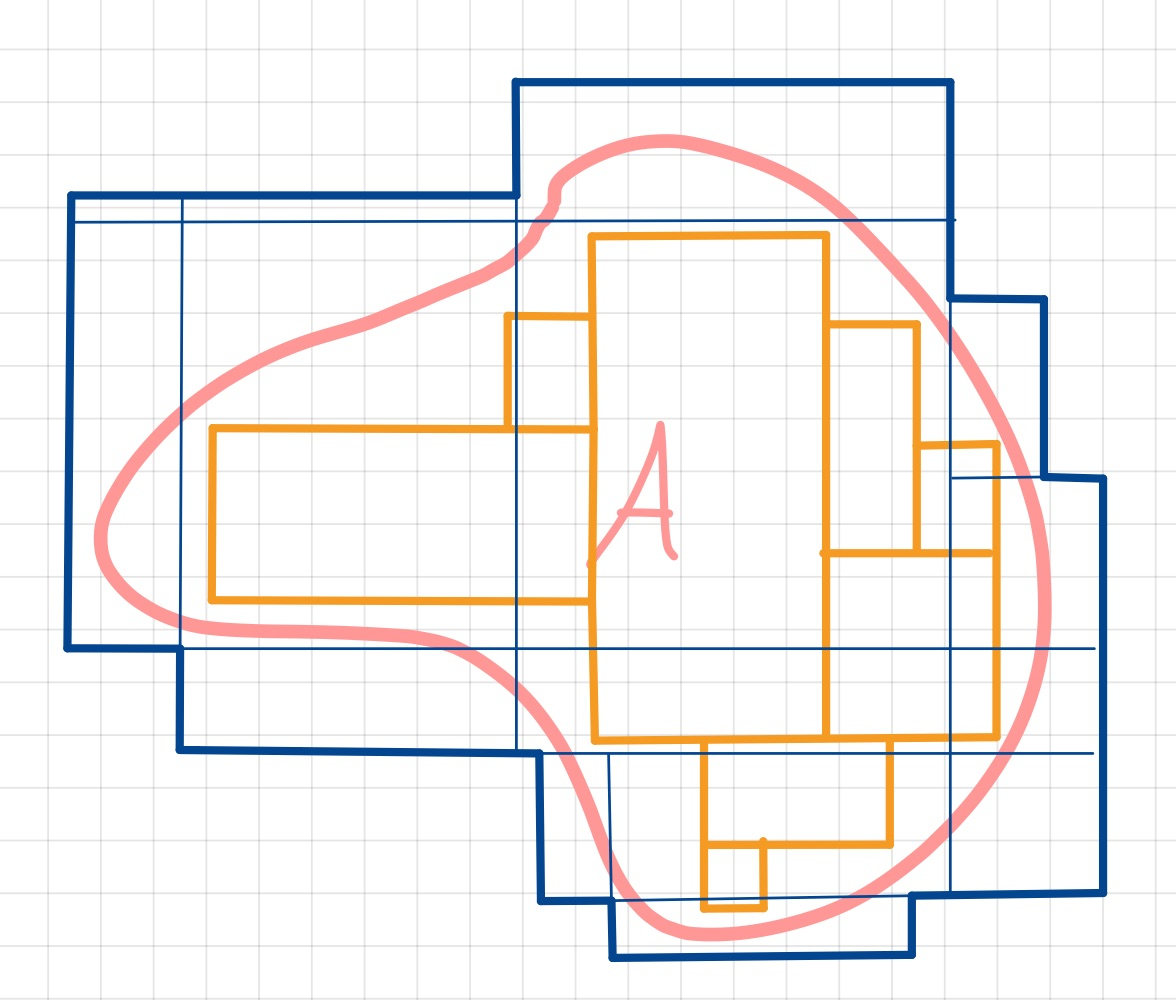
\includegraphics[width=\textwidth]{../\string_build/html/\string_images/jordanmeasure.jpg}
\caption{Visualisierung einer Approximation für das äußere (blau) und das inner (orange) Maß.}\label{\detokenize{masstheorie/masstheorie:fig-jordanmeasure}}\end{figure}

\par
Die Klasse der Jordan messbaren Mengen ist erneut recht klein. Insbesondere hat dieses Konzept erneut Schwierigkeiten mit abzählbar unendlich großen Mengen umzugehen wie folgendes Beispiel zeigt.
\begin{example}{}{masstheorie/masstheorie:ex:jordan}



\par
Wir betrachten die Menge
\begin{align*}
A = (0,1]\cap \mathbb{Q}
\end{align*}
\par
der rationalen Zahlen im Intervall \([0,1]\). Wir betrachten zunächst das äußere Maß und dazu eine Menge
\begin{align*}
J = \bigcup_{i=1}^N Q_i \supset A,
\end{align*}
\par
mit halboffenen Quader \(Q_1,\ldots,Q_N\). Da aber \(J\) und \((0,1]\) jeweils Elemente aus \(\mathcal{R}_{\text{Q}}\) sind gilt auch
\(L = (0,1]\setminus J \in\mathcal{R}\). Wäre nun \(L\) nicht leer, so gäbe es per Definition der halboffenen Quader eine offene Umgebung
\begin{align*}
U\subset L.
\end{align*}
\par
Da aber \(A\) dicht in \((0,1]\) liegt und somit auch \(J\) führt dies auf einen Widerspruch. Deshalb folgt \(L=\emptyset\) und daher
\begin{align*}
(0,1]\subset J \Rightarrow 1\leq \iota^\ast(A).
\end{align*}
\par
Für das innere Maß betrachten wir
\begin{align*}
J = \bigcup_{i=1}^N Q_i \subset A,
\end{align*}
\par
angenommen \(J\) wäre nicht leer, dann folgt dass eine offenen Umgebung \(U\) existiert s.d.
\begin{align*}
U\subset J.
\end{align*}
\par
Da aber auch die irrationalen Zahlen \(\R\setminus \mathbb{Q}\) dicht in \(\R\) liegen folgt daher
\begin{align*}
\left[U\cap\R\setminus \mathbb{Q} \neq \emptyset\right] 
\Rightarrow 
\left[J \cap \R\setminus \mathbb{Q} \neq \emptyset\right]
\Rightarrow 
\left[J\not\subset \mathbb{Q}\right]
\end{align*}
\par
was im Widerspruch zu \(J\subset A\) steht, daher gilt
\begin{align*}
J=\emptyset\Rightarrow \iota_\ast(J) = 0
\end{align*}
\par
und somit
\begin{align*}
\iota_\ast(J) \neq \iota^\ast(J).
\end{align*}\end{example}

\par
Die Menge der Jordan messbaren Mengen bildet weiterhin keine \(\sigma\) Algebra und daher ist der Jordan Inhalt kein Maß im Sinne von \cref{masstheorie/masstheorie:def:mass}  Dies ist an folgendem Beispiel ersichtlich.
\begin{example}{}{masstheorie/masstheorie:example-25}



\par
Wir wollen den Jordan Inhalt einer Punktmengen \(\{a\}\) für \(a\in\R\) berechnen. Mit der Argumentation aus \cref{masstheorie/masstheorie:ex:jordan} erkennen wir, dass das innere Maß gleich null ist, also
\begin{align*}
\iota_\ast(\{a\}) = 0.
\end{align*}
\par
Für das äußere Maß wählen wir eine Folge von offenen Quadern \(Q_i:= (a-1/i, a] \supset \{a\}\) und erkennen, dass
\begin{align*}
\iota^\ast(\{a\})\leq \lim_{i\to\infty} \lambda^n(Q_i) = \lim_{i\to\infty} 1/i = 0
\end{align*}
\par
und damit ist jede Punktmenge Jordan messbar.

\par
Da aber \(\mathbb{Q}\) abzählbar ist, können wir eine Folge \((q_i)_{i\in\N}\) finden, s.d.
\begin{align*}
A = (0,1]\cap \mathbb{Q} = \bigcup_{i\in\N} \{q_i\},
\end{align*}
\par
die Menge \(A\) lässt sich also als abzählbare Vereinigung von Jordan messbaren Mengen darstellen. Aus \cref{masstheorie/masstheorie:ex:jordan} wissen wir aber, dass \(A\) nicht Jordan messbar ist und somit bildet die Klassen der Jordan messbaren Menge \textbf{keine} \(\sigma\) Algebra.
\end{example}


\subsubsection{Das äußere Lebesgue Maß}
\label{\detokenize{masstheorie/masstheorie:das-auszere-lebesgue-masz}}
\par
Wir der letzte Abschnitt zeigt ist der Begriff der Jordan messbarkeit einerseits zu einschränkend (siehe \cref{masstheorie/masstheorie:ex:jordan}  und andererseits führt er nicht auf eine \(\sigma\) Algebra. Wir werden diesen Begriff nun erweitern indem wir uns zunächst nur auf den äußeren Inhalt konzentrieren.

\begin{emphBox}{}{}{Bemerkung:}
\par
Der innere und äußere Inhalt sind intuitiv nicht gleichberechtigt, da das Problem asymmetrisch ist. Konkret ist Subadditivität die inhärente Eigenschaft eines Maßes, da Mengenvereinigungen mehrfach auftretenden Elemente nicht berücksichtigen, während die Addition in \(\R\) für positive Zahlen stets ein größeres Ergebnis liefert. Das äußere Maß ist auf natürliche Weise subadditiv und deshalb zu bevorzugen.
\end{emphBox}
\begin{definition}{}{masstheorie/masstheorie:definition-26}



\par
Das \textbf{äußere Lebesgue Maß} \(\lambda^* \colon 2^{\R^n} \rightarrow [0,\infty]\) ist definiert durch
\begin{align*}
\lambda^*(A) = \inf \left\{ \sum_{k=1}^\infty \mu^n(Q_k) : Q_k \text{ sind halboffene Quader mit } A \subset \bigcup_{k=1}^\infty Q_k \right\}.
\end{align*}\end{definition}

\par
Im Vergleich zum Jordan Inhalt lassen wir nun also unendliche Vereinigungen zu und werten dann Reihen aus über welche das Infimum gebildet wird. Die erste wichtige Aussage in diesem Kontext geht auf Lebesgue zurück. Der Beweis des Satzes benutzt den Satz von Heine Borel.
\begin{theorem}{(Heine Borel)}{masstheorie/masstheorie:thm:heineborel}



\par
Für eine Menge \(\Omega\subset\R^n\) sind die folgenden beiden Aussagen äquivalent:
\begin{enumerate}

\item {} 
\par
\(\Omega\) ist beschränkt und abgeschlossen.

\item {} 
\par
Jede offene Überdeckung von \(\Omega\) enthält eine endliche Teilüberdeckung.

\end{enumerate}
\end{theorem}

\begin{proof}
 Siehe z.B. \cite{For17}.
\end{proof}

\par
Mit diesem Resultat können wir die folgende Aussage beweisen.
\begin{theorem}{}{masstheorie/masstheorie:thm:lebesgue}



\par
Es sei \(J\in\mathcal{R}_{\text{Q}}\) und \((Q_k)_{k\in\N}\) Folge halboffene Quader mit \(J \subset \bigcup_{k=1}^\infty Q_k\).
Dann gilt
\begin{align*}
\lambda^n(J) = \iota(J) = \leq \sum_{k=1}^\infty \lambda^n(Q_k).
\end{align*}\end{theorem}

\begin{proof}
 Wir zeigen die Aussage zunächst für \(J=Q\) wobei \(Q\) ein halboffener Quader ist.

\par
\textbf{Idee:} Verkleinere \(Q\) und vergrößere die \(Q_i\) um Heine Borel anwenden zu können.

\par
Es sei \(\varepsilon>0\) gegeben. Für \(Q=(a,b]\) können wir einen kleineren halboffenen Quader \(Q_\varepsilon\) wählen, s.d.
\begin{align*}
\overline{Q_\varepsilon} \subset Q\\
\lambda^n(Q_\varepsilon) > \lambda^n(Q) - \varepsilon.
\end{align*}
\par
Beachte, dass der Quader so gewählt wird, dass auch sein Abschluss noch in \(Q\) enthalten ist, die zweite Bedingung gibt eine unter Schranke an wie klein der Quader gewählt werden darf. Man kann leicht nachrechnen, dass ein solcher Quader existiert.

\par
Weiterhin wählen wir für jeden Quader \(Q_k\) einen größeren Quader \(Q_k^\varepsilon\), s.d.,
\begin{align*}
\text{Int}(Q_k^\varepsilon)\supset Q_k\\
\lambda^n(Q_k^\varepsilon) < \lambda^n(Q_k) + \frac{\varepsilon}{2^k},
\end{align*}
\par
wobei \(\text{Int}(\cdot)\) das Innere einer Menge bezeichnet.

\par
Mit dieser Konstruktion gilt
\begin{align*}
\overline{Q_\varepsilon} \subset Q\subset \bigcup_{k\in\N} Q_k \subset 
\bigcup_{k\in\N}\text{Int}(Q_k^\varepsilon)
\end{align*}
\par
daher bilden die Mengen \(\text{Int}(Q_k^\varepsilon)\) eine abzählbare offenen Überdeckung der kompakten Menge \(\overline{Q_\varepsilon}\).
Nach dem Satz von Heine Borel (\cref{masstheorie/masstheorie:thm:heineborel}  existiert somit eine endliche Teilüberdeckung und daher ein \(N\in\N\), s.d.,
\begin{align*}
\overline{Q_\varepsilon}\subset \bigcup_{k=1}^N\text{Int}(Q_k^\varepsilon).
\end{align*}
\par
Für endlich viele Quader können wir nun die Eigenschaften aus \cref{masstheorie/masstheorie:thm:lebesguevolume} benutzen und folgern
\begin{align*}
\lambda^n(Q) -\varepsilon &< \lambda^n(Q_\varepsilon) \leq 
\lambda^n\left(\bigcup_{k=1}^N\text{Int}(Q_k^\varepsilon\right) 
\\&\leq 
\sum_{k=1}^N \lambda^n(Q_k^\varepsilon) < 
\sum_{k=1}^N \lambda^n(Q_k) + \frac{\varepsilon}{2^k} 
\\&\leq
\sum_{k=1}^\infty \lambda^n(Q_k) + \frac{\varepsilon}{2^k} = \sum_{k=1}^\infty \lambda^n(Q_k) +\varepsilon.
\end{align*}
\par
Da \(\varepsilon>0\) beliebig war folgt die Aussage indem wir \(\varepsilon\) gegen \(0\) schicken.

\par
Sei nun \(J\in\mathcal{R}_{\text{Q}}\), wobei \(W_1,\ldots,W_N\) paarweise disjunkte halboffene Quader existieren, s.d.,
\begin{align*}
J = \bigcup_{i=1}^N W_i.
\end{align*}
\par
Dann sehen wir, dass für jedes \(i=1,\ldots,N\) die Folge \((Q_k\cap W_i)_{k\in\N}\) erneut eine Folge halboffener Quader mit
\begin{align*}
W_i \subset \bigcup_{k\in\N} Q_k\cap W_i
\end{align*}
\par
ist und daher können wir den ersten Fall anwenden. Somit folgt
\begin{align*}
\iota(J) = \sum_{i=1}^N \lambda^n(W_i) \leq \sum_{i=1}^N \sum_{k=1}^\infty \lambda^n(W_i\cap Q_k) = 
\sum_{k=1}^\infty\sum_{i=1}^N \lambda^n(W_i\cap Q_k) = \sum_{k=1}^\infty \lambda^n(Q_k).
\end{align*}\end{proof}

\par
Analog zum Lebesgue Inhalt auf \(\mathcal{R}_\text{Q}\) in \cref{masstheorie/masstheorie:thm:lebesguevolume} können wir auch für das äußere Lebesgue Maß ähnliche Eigenschaften zeigen.
\begin{theorem}{(Eigenschaften des äußeren Lebesgue Maßes)}{masstheorie/masstheorie:thm:outerlebesgue}



\par
Das äußere Lebesgue Maß \(\lambda^*\) hat folgende Eigenschaften:

\par
1. \(\lambda^*(\emptyset) = 0\)

\par
2. Für zwei Mengen \(A, B \in \R^n\) mit \(A \subset B\) gilt:
\begin{align*}
\lambda^*(A) \leq \lambda^*(B) \qquad (\text{Monotonie}).
\end{align*}
\par
3. Für eine Folge \((A_k)_{k\in\N}\) von Teilmengen des \(\R^n\) gilt:
\begin{align*}
\lambda^*\left( \bigcup_{k=1}^\infty A_k \right) \leq \sum_{k=1}^\infty \lambda^*(A_k) \qquad (\sigma\!-\!\text{Subadditivität}).
\end{align*}
\par
4. Für \(J\in\mathcal{R}_{\text{Q}}\) gilt,
\begin{align*}
\lambda^*(J) = \iota(J).
\end{align*}
\par
5. Für jede Teilmenge \(A \subset \R^n\) und jeden halboffenen Quader \(Q\) gilt:
\begin{align*}
\lambda^*(A) = \lambda^*(A \setminus Q) + \lambda^*(A \cap Q).
\end{align*}\end{theorem}

\begin{proof}
 \textbf{Ad 1.}

\par
Da \(\emptyset\) ein halboffener Quader ist gilt
\begin{align*}
0\leq \lambda^\ast(\emptyset) \leq \lambda^n(\emptyset) = 0.
\end{align*}
\par
\textbf{Ad 2.}

\par
Es bezeichne
\begin{align*}
\mathcal{C}(B) = \{ (Q_i)_{i\in\N}: Q_i \text{ ist halboffener Quader, für }i\in\N, B\subset \bigcup_{i\in\N} Q_i  \}
\end{align*}
\par
die Menge der möglichen Quaderüberdeckungen. Aus \(A\subset B\) folgt dann \(\mathcal{C}(B) \subset \mathcal{C}(A)\), da jede Überdeckung für \(B\) auch eine Überdeckung für \(A\) ist und daher
\begin{align*}
\lambda^\ast(A) = \inf_{\sum_{i=1}^\infty:(Q_i)_{i\in\N}\in \mathcal{C}(A)} \leq 
\inf_{\sum_{i=1}^\infty:(Q_i)_{i\in\N}\in \mathcal{C}(B)} = \lambda^\ast(B).
\end{align*}
\par
\textbf{Ad 3.}

\par
Sei \(\varepsilon>0\) gegeben. Per Definition des Infimums existiert für jede Menge \(A_k\) eine Folge von halboffenen Quadern \(Q_k^i, i\in\N\), s.d.
\begin{align*}
A_k \subset \bigcup_{i\in\N} Q_i\\
\lambda^\ast(A_k) > \sum_{i=1}^\infty \lambda^n(Q_k^i) - \frac{\varepsilon}{2^k}.
\end{align*}
\par
Dann folgt aber auch, dass
\begin{align*}
\bigcup_{k\in\N} A_k \subset \bigcup_{k\in\N}\bigcup_{i\in\N} Q_k^i
\end{align*}
\par
und da die rechte Seite erneut eine Quaderüberdeckung ist folgt per Definition
\begin{align*}
\lambda^\ast\left(\bigcup_{k\in\N} A_k\right) 
&\leq \sum_{k=1}^\infty\sum_{i=1}^\infty \lambda^n(Q_k^i)\\
&<
\sum_{k=1}^\infty \lambda^\ast(A_k) - \frac{\varepsilon}{2^k} =
\sum_{k=1}^\infty \lambda^\ast(A_k) - \varepsilon.
\end{align*}
\par
Die Aussage folgt indem wir \(\varepsilon\) gegen 0 schicken.

\par
\textbf{Ad 4.}

\par
Es sei \(J\in\mathcal{R}_{\text{Q}}\), per Definition folgt direkt
\begin{align*}
\lambda^\ast(Q)\leq \iota^\ast(Q).
\end{align*}
\par
Mit \cref{masstheorie/masstheorie:thm:lebesgue} folgt aber auch
\begin{align*}
\iota^\ast(Q)\leq \lambda^\ast(Q).
\end{align*}
\par
\textbf{Ad 5.}

\par
Es seien zunächst \(A\) und \(Q\) halboffene Quader, dann ist auch \(A\cap Q\) ein halboffener Quader und wir finden paarweise disjunkte halboffene Quader \(Q_0,\ldots,Q_N\), s.d.
\begin{align*}
A\cap Q = Q_0\\
A = \bigcup_{i=1}^N Q_i
\end{align*}
\par
und damit
\begin{align*}
\lambda^n(A) &= \lambda^n\left(\bigcup_{i=0}^N Q_i\right)\\
&= 
\lambda^n(A\cap Q) + \lambda^n\left(\bigcup_{i=1}^N Q_i\right)\\
&\geq \lambda^n(A\cap Q) + \lambda^n(A\setminus Q) \\
&\geq \lambda^n(A).
\end{align*}
\par
Durch die Abschätzung nah oben und nach unten folgt dann
\begin{align*}
\lambda^n(A) = \lambda^n(A\cap Q) + \lambda^n(A\setminus Q).
\end{align*}
\par
Als nächsten Schritt betrachten wir eine Folge halboffener Quader \((Q_i)_{i\in\N}\mathcal{C}(A)\) und erhalten dann
\begin{align*}
\sum_{i=1}^\infty \lambda^n(Q_i) &= 
\sum_{i=1}^\infty \lambda^n(Q_i\cap Q) + \lambda^n(Q_i\setminus Q)\\
&\overset{2.}{\geq}
\lambda^n(A\cap Q) + \lambda^n(A\setminus Q)
&\overset{2.}{\geq}
\lambda^n(A).
\end{align*}
\par
Nehmen wir das Infimum über \(\mathcal{C}(A)\) folgt
\begin{align*}
\lambda^n(A) \geq \lambda^n(A\cap Q) + \lambda^n(A\setminus Q) \geq 
\lambda^n(A)
\end{align*}
\par
und daher die Behauptung.
\end{proof}

\par
Als Korollar von \cref{masstheorie/masstheorie:thm:lebesgue} und den vorherigen Eigenschaften erhalten wir eine Abschätzung für das äußere Lebesgue Maß sowohl von oben durch den äußeren Jordan Inhalt als auch von unten durch den inneren Jordan Inhalt.
\label{masstheorie/masstheorie:corollary-30}
\begin{emphBox}{}{}{Corollary 5.1}



\par
Es sei \(A\subset\R^n\), dann gilt
\begin{align*}
\iota_\ast(A) \leq \lambda^\ast(A) \leq \iota^\ast(A).
\end{align*}\end{emphBox}

\begin{proof}
 Für jedes Element \(J\in\mathcal{R}_{\text{Q}}\) und beliebige halboffene Quader \(Q_i,\i\in\N\), s.d.,
\begin{align*}
J\subset A\subset \bigcup_{i\in\N} Q_i
\end{align*}
\par
folgt aus \cref{masstheorie/masstheorie:thm:lebesgue} \begin{align*}
\lambda^n(J)\leq \sum_{i=1}^\infty Q_i.
\end{align*}
\par
Dies gilt für jedes \(J\in \mathcal{R}_{\text{Q}}\) mit \(J\subset A\) und daher insbesondere auch für das Supremum, daher
\begin{align*}
\iota_\ast(A) \leq \sum_{i=1}^\infty Q_i.
\end{align*}
\par
Diese Aussage gilt wiederum für eine beliebige Folge halboffener Quader welche \(A\) überdecken und daher auch für das Infimum, also
\begin{align*}
\iota_\ast(A) \leq \lambda^\ast(A).
\end{align*}
\par
Die andere Ungleichung folgt per Definition da jede endliche Überdeckung mit halboffenen Quadern (welche im Infimum für \(\iota^\ast\) betrachtet werden) auch im Infimum über abzählbare Überdeckungen berücksichtigt wird, daher
\begin{align*}
\lambda^\ast(A)\leq\iota^\ast(A).
\end{align*}\end{proof}

\par
Die obige Eigenschaft liefert zusätzlich die Aussage, dass für Jordan messbare Mengen \(A\) gilt
\begin{align*}
\iota(A)\leq\lambda^\ast(A)\leq\iota(A)\Rightarrow \lambda^\ast(A) = \iota(A).
\end{align*}\begin{remark}{(Wirkung von Transformationen auf das äußere Lebesgue Maß)}{masstheorie/masstheorie:rem:transinvariance}



\par
Eine besondere Eigenschaft des äußeren Lebesgue Maßes ist es, dass es \emph{bewegungsinvariant} ist, d.h., dass es unter Translationen und Rotationen den gleichen Wert behält.
Dies ist für viele Anwendungen eine fundamentale Eigenschaft.
Die folgende Bemerkung hält die Wirkung von geometrischen Transformationen auf das äußere Lebesgue Maß fest.

\par
1. Sei \(A \subset \R^n\) eine beliebige Teilmenge und \(a \in \R^n\) ein beliebiger Vektor.
Dann ist das äußere Lebesgue Maß \textbf{translationsinvariant} unter der Wirkung von \(a\), d.h., es gilt
\begin{align*}
\lambda^*(A + a) = \lambda^*(A).
\end{align*}
\par
Außerdem gilt, dass die Teilmenge \(A\) genau dann Lebesgue messbar ist, wenn die verschobene Teilmenge \(A + a\) Lebesgue messbar ist.

\par
2. Sei \(A \subset \R^n\) eine beliebige Teilmenge und \(M \in \R^{n\times n}\) eine beliebige Matrix.
Dann gilt für das äußere Lebesgue Maß der folgende Zusammenhang unter der Wirkung der linearen Transformation \(M\)
\begin{align*}
\lambda^*(MA) = |\!\operatorname{det}(M)| \, \lambda^*(A).
\end{align*}
\par
Das heißt insbesondere, dass das äußere Lebesgue Maß invariant unter Transformationen der orthogonalen Gruppe (z.B. \textbf{Rotationen} und \textbf{Spiegelungen}) ist, da für diese Transformationen \(|\!\operatorname{det}(M)| = 1\) gilt (siehe Kapitel 3.6 in \cite{Ten21}).

\par
Außerdem gilt, dass die Teilmenge \(A\) genau dann Lebesgue messbar ist, wenn die linear transformierte Teilmenge \(MA\) Lebesgue messbar ist.
\end{remark}


\subsubsection{Nullmengen}
\label{\detokenize{masstheorie/masstheorie:nullmengen}}
\par
Eine relevante Klasse von Teilmengen des \(\R^n\) bilden sogenannten \textbf{Lebesgue Nullmengen}.
\begin{definition}{}{masstheorie/masstheorie:definition-32}



\par
Eine Teilmenge \(N \subset \R^n\) eine \textbf{(Lebesgue )Nullmenge}, falls ihr äußeres Lebesgue Maß Null ist, d.h., es gilt
\begin{align*}
\lambda^*(N) = 0.
\end{align*}\end{definition}

\par
Für die Klasse der Nullmengen können wir folgende Eigenschaften zeigen.
\begin{lemma}{(Eigenschaften von Lebesgue Nullmengen)}{masstheorie/masstheorie:lem:eigenschaftenNullmengen}



\par
Für Lebesgue Nullmengen gelten die folgenden Eigenschaften:
\begin{enumerate}

\item {} 
\par
Sei \((N_n)_{n\in\N}\) eine Familie von Nullmengen.
Dann ist auch \(\bigcup_{n\in\N} N_n\) eine Nullmenge.

\item {} 
\par
Alle abzählbaren Mengen sind Nullmengen.

\item {} 
\par
Alle Teilmengen von Nullmengen sind Nullmengen.

\end{enumerate}
\end{lemma}

\begin{proof}
 

\par
\textbf{Ad 1.}

\par
Auf Grund der \emph{\(\sigma\) Subadditivität} des äußeren Lebesgue Maßes folgt direkt
\begin{align*}
0 \leq \mu^* \left( \bigcup_{n\in\N} N_n \right) \leq \sum_{n\in\N} \mu^*(N_n) = 0.
\end{align*}
\par
Da \(\mu^* \left( \bigcup_{n\in\N} N_n \right)\) gilt ist also \(\bigcup_{n\in\N} N_n\) auch eine Nullmenge.

\par
\textbf{Ad 2.}

\par
Es sei \(A\subset\R^d\) eine abzählbare Menge, d.h., es existiert eine Folge \((a_k)_{k\in\N}\subset\R^d\), s.d.,
\begin{align*}
A = \bigcup_{k\in\N} a_k.
\end{align*}
\par
Es sei nun \(\varepsilon>0\) gegeben, dann wählen wir die Folge halboffener Quader
\begin{align*}
Q_k := (a_k - \frac{\varepsilon}{2^k},a_k]
\end{align*}
\par
s.d.,
\begin{align*}
A\subset \bigcup_{k\in\N} Q_k.
\end{align*}
\par
Dann folgt aber,
\begin{align*}
\lambda^\ast(A) \leq \sum_{k\in\N} \lambda^n(Q_k) = \sum_{k\in\N} \frac{\varepsilon}{2^k} = \varepsilon.
\end{align*}
\par
Wir können nun \(\varepsilon\) gegen 0 schicken und erhalte die Aussage.

\par
\textbf{Ad 3.}

\par
Es sei \(N\) eine Nullmenge und \(A\subset N\), dann folgt aus der Monotonie
\begin{align*}
0\leq \lambda^\ast(A)\leq \lambda^\ast(N) = 0.
\end{align*}\end{proof}

\par
Intuitiv könnten man meinen, dass lediglich abzählbare MEngen Lebesgue Nullmengen sind, dies ist jedoch nicht der Fall. Ein Beispiel ist die \href{https://de.wikipedia.org/wiki/Cantor-Menge}{canto Menge} welche überabzählbar ist, aber Lebesgue Maß null hat.


\subsubsection{Das äußere Maß ist kein Maß}
\label{\detokenize{masstheorie/masstheorie:das-auszere-masz-ist-kein-masz}}\label{\detokenize{masstheorie/masstheorie:s-vitali}}
\par
Für das äußere Lebesgue Maß kann man einige Eigenchaften zeigen (siehe \cref{masstheorie/masstheorie:thm:outerlebesgue}  welche zwar eine Maß erinnern. Der größte Unterschied bisher ist, dass wir nur \(\sigma\) Subadditivität und nicht \(\sigma\) Additivität zeigen konnten. Insbesondere arbeitet das äußere Maß auf der gesamten Potenzmenge \(2^{\R^d}\) und nicht auf einer kleineren \(\sigma\) Algebra, man könnte also vermuten, dass diese Menge zu groß ist um \(\sigma\) Additivität zeigen zu können, was tatsächlich der Fall ist.

\par
Um das zu sehen betrachten wir die sogenannte Vitali Menge auf \(\R\).

\begin{emphBox}{Giuseppe Vitali}{}

\par
\href{https://de.wikipedia.org/wiki/Giuseppe\_Vitali}{Giuseppe Vitali} (geboren 26. August 1875 in Ravenna; gestorben 29. Februar 1932 in Bologna) war ein italienischer Mathematiker.
\end{emphBox}

\par
Für zwei Punkte \(x,y\in\R\) definiert man die Äquivalenzrelation
\begin{align*}
x \sim y \quad \Leftrightarrow \quad x-y \in \Q.
\end{align*}
\par
d.h. zwei Punkte gehören der selben Äquivalenzklasse an sofern ihre Differenz rational ist. Es gilt also
\begin{align*}
[x] = \{y: y-x\in\Q\}
\end{align*}
\par
jede Klasse \([x]\) ist abzählbar und \([0] = \Q\). Falls \([x]\cap [y]\neq \emptyset\), so folgt, dass ein \(z\in[x]\cap [y]\) existiert und damit
\begin{align*}
\left.
\begin{matrix}
z-x\in\Q\\
z-y\in\Q\\
\end{matrix}
\right\}
\Rightarrow x-y\in\Q\Rightarrow [x]=[y],
\end{align*}
\par
daher sind zwei Äquivalenzklassen entweder gleich oder disjunkt. Da aber
\begin{align*}
\R = \bigcup_{x\in\R} [x]
\end{align*}
\par
gilt, muss es überabzählbar viele disjunkte Äquivalenzklassen geben, ansonsten wäre \(\R\) selbst abzählbar. Mithilfe des \href{https://de.wikipedia.org/wiki/Auswahlaxiom}{Auswahl Axioms} können wir nun für jede einzelne Äquivalenzklasse einen Repräsentanten wählen, wobei wir die Menge der Repräsentanten \(V\) als \textbf{Vitali Menge} bezeichnen. Zwei Elemente \(x,y\in V, x\neq y\) unterscheiden sich stets um eine irrationale Zahl, denn
\begin{align*}
x-y\in\Q \Rightarrow [x] = [y]
\end{align*}
\par
ist ein Widerspruch zur Konstruktion.

\par
Es sei nun \((q_k)_{k\in\N}\) eine Abzählung der rationalen Zahlen und definiere die verschobenen Vitali Mengen
\begin{align*}
V_k :=\{x+q_k: x\in V\}.
\end{align*}\begin{lemma}{}{masstheorie/masstheorie:lemma-34}



\par
Mit den obigen Definitionen gilt
\begin{enumerate}

\item {} 
\par
\(\lambda^\ast(V) = \lambda^\ast(V_k)\) für alle \(k\in\N\),

\item {} 
\par
\(V_k\cap V_l=\emptyset\) für \(k\neq l\),

\item {} 
\par
\(\bigcup_{k\in\N} V_k = \R\).

\end{enumerate}
\end{lemma}

\begin{proof}
 

\par
\textbf{Ad 1.}

\par
Diese Tatsache folgt, da das äußere Lebesgue Maß Translationsinvariant ist, siehe \cref{masstheorie/masstheorie:rem:transinvariance} 

\par
\textbf{Ad 2.}

\par
Für \(x,y\in V\) gilt
\begin{align*}
x + q_k = y + q_l&\Rightarrow x-y\in\Q\\
\Rightarrow [x]=[y]&\Rightarrow x=y\\
\Rightarrow q_k=q_l&\Rightarrow k=l
\end{align*}
\par
wobei wir in der zweiten Zeile erneut ausnutzen, dass die Elemente aus \(V\) jeweils disjunkte Äquivalenzklassen erzeugen.

\par
\textbf{Ad 3.}

\par
Trivialerweise gilt
\begin{align*}
\bigcup_{k\in\N} V_k \subset \R.
\end{align*}
\par
Andererseits sei \(x\in\R\) dann existiert \(v\in V\) s.d. \([v] = [x]\). Somit gilt \(x-v\in\Q\) und es existiert \(k\in\N\), s.d.
\begin{align*}
q_k = x-v.
\end{align*}
\par
Somit folgt \(x=v+q_k\in V_k\) und daher \(x\in\bigcup_{k\in\N} V_k\).
\end{proof}

\par
Mithilfe einer Vitali Menge können wir nun die \(\sigma\) Additivität des äußeren Lebesgue Maßes zum Widerspruch führen.
\begin{lemma}{}{masstheorie/masstheorie:lemma-35}



\par
Das äußere Lebesgue Maß \(\lambda^\ast\) ist nicht \(\sigma\) Additiv auf \(2^{\R}\).
\end{lemma}

\begin{proof}
 \textbf{Annahme}: Das äußere Lebesgue Maß sei \(\sigma\) Additiv auf \(2^{\R}\).

\par
Die Mengen \(V_k\) sind paarweise disjunkt und überdecken \(\R\), daher folgt
\begin{align*}
0<\lambda^\ast(\R) = \lambda^\ast(\bigcup_{k\in\N} V_k) = \sum_{k\in\N} \lambda^\ast(V_k) = \sum_{k\in\N} \lambda^\ast(V)
\end{align*}
\par
und daher \(\lambda^\ast(V)>0\). Diese Folgerung wollen wir nun zum Widerspruch führen. Dazu betrachten wir die folge halboffener Quader \(Q_k:=(k,k]\) und erkennen unter Ausnutzung \textbf{endlicher} Additivität, dass
\begin{align*}
\lambda^\ast(V) \geq \lambda^\ast\left(V \cap \bigcup_{k=1}^N Q_k\right) = 
\sum_{k=1}^N \lambda^\ast(V\cap Q_k).
\end{align*}
\par
Somit folgt mithilfe der \(\sigma\) Subadditivität
\begin{align*}
\lambda^\ast(V) \geq \sum_{k=1}^\infty \lambda^\ast(V\cap Q_k) \geq
\lambda^\ast\left(\bigcup_{k\in\N} V\cap Q_k\right) = \lambda^\ast(V).
\end{align*}
\par
Da wir \(\lambda^\ast(V)>0\) folgern konnten, muss daher ein \(N\in\N\) existieren, s.d.,
\begin{align*}
\lambda^\ast(V\cap Q_N) >0.
\end{align*}
\par
Analog zum Beweis, dass die \(V_k\) paarweise disjunkt sind, folgert man auch, dass die Mengen \(\frac{1}{m}+(V\cap Q_N)\) für verschieden \(m\in\N\) paarweise disjunkt sind und wegen der Translationsinvarianz folgt
\begin{align*}
\lambda^\ast(\frac{1}{m}+(V\cap Q_N)) = \lambda^\ast((V\cap Q_N)) >0.
\end{align*}
\par
Wir erkennen allerdings, dass
\begin{align*}
\bigcup_{m\in\N} \frac{1}{m}+(V\cap Q_N) \subset (-N,N+1]
\end{align*}
\par
und nutzen wir nun erneut die angenommene \(\sigma\) Additivität so erhalten wir
\begin{align*}
\infty = \sum_{m=1}^\infty \lambda^\ast(\frac{1}{m}+(V\cap Q_N)) = 
\lambda^\ast\left(\bigcup_{m\in\N}  \frac{1}{m}+(V\cap Q_N) \right)\leq 
\lambda^\ast((-N,N+1]) = 2N + 1
\end{align*}
\par
und somit
\begin{align*}
\infty \leq 2N + 1
\end{align*}
\par
was ein Widerspruch ist. Daher ist die Annahme der \(\sigma\) Additivität falsch.
\end{proof}

\par
Ähnliche Konstruktionen können auch allgemein für \(\R^n\) durchgeführt werden. Man hat allgemein die Aussage, dass \(\lambda^\ast\) auf \(\R^n\) \textbf{kein} Maß ist.


\subsubsection{Das Lebesgue Maße}
\label{\detokenize{masstheorie/masstheorie:das-lebesgue-masze}}
\par
Der vorherige Abschnitt zeigt, dass die Potenzmenge \(2^{\R^n}\) zu groß ist, d.h. auf dieser \(\sigma\) Algebra ist \(\lambda^\ast\) kein Maß. Deshalb wollen wir nun eine Klasse messbarer Mengen definieren, welche dann eine kleinere \(\sigma\) Algebra liefert.
\begin{remark}{(Das Jordan Konzept)}{masstheorie/masstheorie:remark-36}



\par
Eine mögliche Idee um messbare Mengen zu definieren haben wir bereits beim Jordan Inhalt kennengelernt. Hierbei wird zusätzlich zum äußeren Maß ein inneres Maß definiert. Beim Übergang vom äußeren Jordan Inhalt zum äußeren Lebesgue Maß werden endliche Vereinigungen durch unendliche ersetzt, weshalb man versuchen könnte, das nun auch hier zu tun, indem man das innere Lebesgue Maß auch über unendliche Vereinigungen definiert
\begin{align*}
\lambda_\ast(A) := \sup\left\{\sum_{i=1}^\infty Q_i: \bigcup_{i\in\N} Q_i \subset A, Q_i\text{ disjunkte halboffener Quader}\right\}.
\end{align*}
\par
Offensichtlich folgt mit dieser Definition
\begin{align*}
\iota_\ast(A)\leq \lambda_\ast(A)
\end{align*}
\par
da das Supremum über mehr Ausschöpfungen gebildet wird. Nun sei aber \(Q_i\) eine beliebiger Folge halboffener Quader, welche \(A\) von innen ausschöpfen, dann gilt für jedes \(N\in\N\)
\begin{align*}
\iota_\ast(A) \geq \sum_{i=1}^N \lambda^n(Q_i)
\end{align*}
\par
und daher
\begin{align*}
\iota_\ast(A)\geq \sum_{i=1}^\infty \lambda^n(Q_i).
\end{align*}
\par
Diese Ungleichung erhalten wir deshalb so einfach, da für jedes \(N\in\N\) auch \(\bigcup_{i=1}^N Q_i\subset A\) gilt. Beim äußern Maßen konnten wir aber andersherum nicht einfach aus \(A\subset \bigcup_{i=1}^\infty W_i\) auch \(A\subset \bigcup_{i=1}^N W_i\) folgern.

\par
Da die obige Ungleichung für beliebig Folgen halboffener Quader gilt, folgt
\begin{align*}
\iota_\ast(A) \geq \lambda_\ast(A).
\end{align*}
\par
Wir erkennen also, dass für das innere Maß keinen Unterschied macht ob wir endliche oder unendliche Vereinigungen betrachten.

\par
Würden wir Messbarkeit über die Bedingung
\begin{align*}
\lambda_\ast(A)=\lambda^\ast(A)
\end{align*}
\par
definieren erhielten wir erneut keine \(\sigma\) Algebra. Denn für die Menge \(A=[0,1]\setminus\Q\) gilt
\begin{align*}
J\in\mathcal{R}_{\text{Q}}, J\subset A\Rightarrow J=\emptyset
\end{align*}
\par
und daher \(\lambda_\ast(J) = 0\). Der Trick die Menge mit kleinen Quadern zu approximieren wie beim äußeren Maß funktioniert auch nicht, da wir in diesem Fall jeweils die Teilmengen Bedingung verletzt wäre.

\par
Es gilt aber
\begin{align*}
\lambda^\ast(A) = \lambda^\ast([0,1]) - \underbrace{\lambda^\ast(\Q)}_{=0} = 1
\end{align*}
\par
und daher wäre \(A\) nicht messbar, obwohl sowohl \(\Q\), als auch \([0,1]\) messbar wären. Damit hätten wir erneut keine \(\sigma\) Algebra konstruiert.
\end{remark}

\par
Es gibt verschiedene Ansätze Lebesgue Messbarkeit zu definieren (welche alle äquivalent sind), wir wählen im Folgenden das Konzept von
Carathéodory.

\begin{emphBox}{Constantin Carathéodory}{}

\par
\href{https://de.wikipedia.org/wiki/Constantin\_Carath\%C3\%A9odory}{Constantin Carathéodory} (Geboren 13. September 1873 in Berlin; Gestorben 2. Februar 1950 in München) war ein Mathematiker griechischer Herkunft.
\end{emphBox}
\begin{definition}{}{masstheorie/masstheorie:definition-37}



\par
Wir nennen eine Teilmenge \(A \subset \R^n\) \textbf{Lebesgue messbar}, genau dann wenn für alle Teilmengen \(E \subset \R^n\) gilt:
\begin{align*}
\lambda^*(E) = \lambda^*(E \cap A) + \lambda^*(E \setminus A).
\end{align*}
\par
Wir notieren die Menge der Lebesgue messbaren Mengen als
\begin{align*}
\mathcal{A}(\R^n) = \lbrace A \subset \R^n : A \text{ ist Lebesgue-messbar } \rbrace
\end{align*}
\par
Wir definieren das \textbf{Lebesgue Maß} \(\lambda \colon \mathcal{A} \rightarrow [0,\infty]\) messbarer Mengen durch
\begin{align*}
\lambda(A) = \lambda^*(A).
\end{align*}\end{definition}
\begin{remark}{}{masstheorie/masstheorie:remark-38}



\par
Es ist wichtig zu bemerken, dass diese Bedingung eine Einschränkung ist, da das äußere Lebesgue Maß \textbf{nicht} additiv ist auf \(2^{\R^n}\), es gilt lediglich
\begin{align*}
\lambda^*(E) \leq \lambda^*(E \cap A) + \lambda^*(E \setminus A).
\end{align*}
\par
für alle \(A,E\subset\R^d\). Aus diesem Grund scheint die Einschränkung sinnvoll zu sein um Additivität zu erhalten.
\end{remark}

\par
Wir betrachten im Folgenden verschiedene Beispiele messbarer Mengen, was zeigt, dass \(\mathcal{A}\neq \emptyset\).
\begin{lemma}{}{masstheorie/masstheorie:thm:lebesguemes}


\begin{enumerate}

\item {} 
\par
Jede Lebesgue Nullmenge ist Lebesgue messbar, insbesondere ist \(\emptyset\) Lebesgue messbar.

\item {} 
\par
Jeder halboffene Quader ist messbar.

\end{enumerate}
\end{lemma}

\begin{proof}
 ** Ad 1.**

\par
Es sei \(N\) eine Lebesgue Nullmenge und \(E\subset\R^d\), dann gilt
\begin{align*}
\lambda^\ast(E) \leq \underbrace{\lambda^\ast(E\cap\N)}_{=0} + \lambda^\ast(E\setminus N)\leq
 \lambda^\ast(E)
\end{align*}
\par
und daher \(\lambda^\ast(E) = \lambda^\ast(E\cap\N) + \lambda^\ast(E\setminus N)\).

\par
\textbf{Ad 2.}

\par
Folgt aus \cref{masstheorie/masstheorie:thm:outerlebesgue} Eigenschaft 4.
\end{proof}

\par
Weiterhin erhält man über den Begriff der Lebesgue messbarkeit endlich die erhoffte \(\sigma\) Algebra Struktur.
\begin{lemma}{}{masstheorie/masstheorie:lemma-40}



\par
Die Klasse der Lebesgue messbaren Mengen \(\mathcal{A}\) bildet eine \(\sigma\) Algebra.
\end{lemma}

\begin{proof}
 1. Von \cref{masstheorie/masstheorie:thm:lebesguemes} erhalten wir zunächst, dass \(\emptyset\in\mathcal{A}\).

\par
2. Weiterhin sei \(A\in\mathcal{A}\) messbar und \(E\subset\R^d\) beliebig, dann gilt
\begin{align*}
\lambda^\ast(E) = \lambda^\ast(\underbrace{A\cap E}_{=E\setminus A^C}) + \lambda^\ast(\underbrace{E\setminus A}_{=E\cap A^C}) = 
\lambda^\ast(E\setminus A^C) + \lambda^\ast(E\cap A^c)\end{align*}
\par
und daher ist auch \(A^C\in\mathcal{A}\).

\par
3. Wir zeigen zunächst, dass \(\mathcal{A}\) unter endlichen Vereinigungen, Schnitten und Differenzen abgeschlossen ist.

\par
Es seien \(A,B\in\mathcal{A}\) und \(E\subset\R^d\) dann gilt
\begin{align*}
\lambda^\ast(E) &= \lambda^\ast(E\cap A) + \underbrace{\lambda^\ast(E\setminus A)}_{\text{wende Messbarkeit von} B\text{ an}}\\
&=\lambda^\ast(E\cap A) + \lambda^\ast((E\setminus A)\cap B) + \lambda^\ast((E\setminus A)\setminus B)\\
&=
\underbrace{\lambda^\ast(E\cap (A\cup B)\cap A) + \lambda^\ast((E\cap A\cup B)\setminus A)}_{\text{wende Messbarket von } A \text{ an}} + \lambda^\ast(E\setminus(A\cup B))\\
&=
\lambda^\ast(E\cap (A\cup B)) + \lambda^\ast(E\setminus(A\cup B))
\end{align*}
\par
und daher ist \(A\cup B\) messbar. Weiterhin folgt \(A\cap B = (A^C\cup B^C)^C\in\mathcal{A}\) und daher auch \(A\cap B\in\mathcal{A}\). Außerdem gilt \(A\setminus B = A\cap B^C\) und somit auch \(A\setminus B\in\mathcal{A}\).

\par
4. Sei nun \(A_i\in\mathcal{A}\) für \(i\in\N\) eine \textbf{disjunkte} Folge von Mengen und setze \(A=\bigcup_{i\in\N} A_i\). Unter Ausnutzung von \(A_1\in\mathcal{A}\) haben wir für \(E\subset\R^d\)
\begin{align*}
\lambda^\ast(E\cap (A_1\cup A_2)) &= \lambda^\ast(E\cap(A_1\cup A_2)\cap A_1) + \lambda^\ast(E\cap(A_1\cup A_2)\setminus A_1)\\
&=
\lambda^\ast(E\cap A_1) + \lambda^\ast(E\cap A_2)
\end{align*}
\par
und somit gilt für endliche Vereinigungen
\begin{align*}
\lambda^\ast(E\cap \bigcup_{i=1}^N A_i) = \sum_{i=1}^N \lambda^\ast(E\cap A_i).
\end{align*}
\par
Mit Monotonie folgt dann für jedes \(N\in\N\)
\begin{align*}
\lambda^\ast(E\cap A)\geq \lambda^\ast(E\cap \bigcup_{i=1}^N A_i) = \sum_{i=1}^N \lambda^\ast(E\cap A_i)
\end{align*}
\par
und daher mit der \(\sigma\) Subadditivität
\begin{align}\label{equation:masstheorie/masstheorie:eq:LebesgueAlgebra}
\lambda^\ast(E\cap A) \geq \sum_{i=1}^\infty \lambda^\ast(E\cap A_i)\geq \lambda^\ast\left(\bigcup_{i\in\N} E\cap A_i\right) = \lambda^\ast(E\cap A).
\end{align}
\par
Weiterhin wissen wir nach 3., dass endliche Vereinigungen messbarer Mengen messbar sind, daher
\begin{align*}
\lambda^\ast(E) &= \lambda^\ast\left(E\cap \bigcup_{i=1}^N A_i\right) + \lambda^\ast\left(E\setminus \bigcup_{i=1}^N A_i\right)\\
&\geq
\sum_{i=1}^N \lambda^\ast(E\cap A_i) + \lambda^\ast(E\setminus A)
\end{align*}
\par
für alle \(N\in\N\) und somit
\begin{align*}
\lambda^\ast(E)\geq \sum_{i=1}^\infty \lambda^\ast(E\cap A_i) + \lambda^\ast(E\setminus A)\geq 
\lambda^\ast(E\cap A) + \lambda^\ast(E\setminus A) \geq \lambda^\ast(E).
\end{align*}
\par
Daraus schließen wir mit , dass {\color{red}\bfseries{}:eqref:`eq:LebesgueAlgebra`}
\begin{align*}
\lambda^\ast(E) = \sum_{i=1}^\infty \lambda^\ast(E\cap A_i) + \lambda^\ast(E\setminus A) =
\lambda^\ast(E\cap A) + \lambda^\ast(E\setminus A).
\end{align*}
\par
5.\textbackslash{} Es bleibt die Aussage für eine belibige nicht notwendigerweise disjunkte Folge \(A_i\in\mathcal{A}, i\in\N\) zu zeigen. Dazu definieren wir die Mengen \(B_1:=A_1\),
\begin{align*}
B_k := A_i\setminus \left(\bigcup_{i=1}^k B_i  \right)
\end{align*}
\par
wobei wir erkennen, dass die \(B_i\) paarweise disjunkt sind und insbesondere gilt
\begin{align*}
\bigcup_{k\in\N} B_k = \bigcup_{i\in\N} A_i.
\end{align*}
\par
Nach 4. ist damit auch diese Vereinigung messbar.
\end{proof}

\par
Mit dieser Aussage können wir weitere messbare Mengen identifizieren.
\begin{lemma}{}{masstheorie/masstheorie:thm:lebesgueOffenAbgeschlossen}



\par
Offene und abgeschlossene Teilmengen des \(\R^n\) sind Lebesgue messbar.
\end{lemma}

\begin{proof}
 Es sei \(U\subset\R^d\) offen, wir betrachten die Menge
\begin{align*}
\bigcup_{a,b\in \Q^d, (a,b]\subset U} (a,b]\subset U
\end{align*}
\par
Sei nun \(x\in U\), dann existiert auch \(a,b\in\Q^d\), s.d. \(x\in(a,b]\subset U\) und somit \(x\in\bigcup_{a,b\in \Q^d, (a,b]\subset U}\), woraus wir schließen
\begin{align*}
\bigcup_{a,b\in \Q^d, (a,b]\subset U} (a,b] = U.
\end{align*}
\par
Somit ist \(U\) abzählbare Vereinigung messbarer Mengen und daher selbst messbar.

\par
Abgeschlossene Mengen sind als Komplemente offener und daher messbarer Mengen, selbst messbar.
\end{proof}

\par
Da wir nun eine \(\sigma\) Algebra zu Verfügung haben können wir ein Maß definieren.
\begin{definition}{}{masstheorie/masstheorie:definition-42}



\par
Wir definieren das Lebesgue Maß \(\lambda^n:\mathcal{A}\to[0,\infty]\) über die Einschränkung des äußeren Maßes, d.h.,
\begin{align*}
\lambda^n(A):= \lambda^\ast(A)\text{ für } A\in\mathcal{A}.
\end{align*}\end{definition}

\begin{emphBox}{}{}
\par
ToDo
\end{emphBox}
\begin{theorem}{(Regularität des Lebesgue Maßes)}{masstheorie/masstheorie:theorem-43}



\par
Das Lebesgue Maß ist von außen und innen regulär im Sinne von \cref{masstheorie/masstheorie:def:regularitaet}  d.h., für jede Lebesgue messbare Teilmenge \(A \subset \R^n\) gilt

\par
1. für jedes \(\epsilon > 0\) existiert eine offene Menge \(U\) mit \(A \subset U\) für die gilt \(\mu(U \setminus A) < \epsilon\),

\par
2. für jedes \(\epsilon > 0\) existiert eine abgeschlossene Menge \(F\) mit \(F \subset A\) für die gilt \(\mu(A \setminus F) < \epsilon\).
\end{theorem}

\begin{proof}
 ToDo.
\end{proof}
\begin{theorem}{(Charakterisierung Lebesgue messbarer Mengen)}{masstheorie/masstheorie:theorem-44}



\par
Die folgenden drei Aussagen sind äquivalent, so dass sie eine Charakterisierung der Lebesgue messbaren Mengen darstellen.

\par
1. Eine Teilmenge \(A \subset \R^n\) ist Lebesgue messbar.

\par
2. Für jedes \(\epsilon > 0\) existiert eine offene Menge \(U\) und eine abgeschlossene Menge \(F\), so dass \(F \subset A \subset U\) und es gilt \(\mu(U \setminus F) < \epsilon\).

\par
3. Für jedes \(\epsilon > 0\) existiert eine offene Menge \(U\) mit \(A \subset U\) für die gilt \(\mu(U \setminus A) < \epsilon\).
\end{theorem}

\begin{proof}
 ToDo
\end{proof}

\par
Man kann für die Borel \(\sigma\) Algebra von \(\R^n\) zeigen, dass gilt
\begin{align*}
\B(\R^n) = \sigma(\lbrace A \subset \R^n \text{ offen }\rbrace) ) = \sigma(\lbrace A \subset \R^n \text{ abgeschlossen }\rbrace)
\end{align*}
\par
Die letzte Gleichung gilt, da \(\sigma\) Algebren abgeschlossen unter Komplementbildung sind.
Zusammen mit \cref{masstheorie/masstheorie:thm:lebesgueOffenAbgeschlossen} folgt dann schon, dass die Borel \(\sigma\) Algebra \(\B(\R^n)\) eine Teilmenge der Lebesgue messbaren Mengen ist.
Der folgende Satz zeigt, dass es eine echte Teilmenge ist indem er den Unterschied der Mengen als Lebesgue Nullmengen charaterisiert.
\begin{theorem}{}{masstheorie/masstheorie:theorem-45}



\par
Eine Teilmenge \(A \subset \R^n\) ist genau dann Lebesgue messbar, wenn eine Teilmenge \(B \in \B(\R^n)\) und eine Nullmenge \(N \subset \R^n\) existiert, so dass \(A = B \cup N\) ist, wobei \(B\cap N=\emptyset\).
\end{theorem}

\begin{proof}
 ToDo
\end{proof}


\section{Lebesgue Integral}
\label{\detokenize{masstheorie/lebesgue_integral:lebesgue-integral}}\label{\detokenize{masstheorie/lebesgue_integral::doc}}
\par
Anhand des in \cref{masstheorie/masstheorie:s-lebesguemeasure}  konstruirten Maßes wollen wir nun einen neuen Begriff des Integrals herleiten. Unsere Motivation hierbei war anstatt den Definitionsbereich, den Bildbereich einer Funktion \(f:\Omega\to\R\) zu zerteilen. Dies führt auf das Problem, dass man Urbildern
\begin{align*}
f^{-1}(I)
\end{align*}
\par
für Mengen \(I\subset\R\) ein Maß zuordnen muss. Dies soll im Folgenden mithilfe des Lebesgue Maßes geschehen. Um \(f^{-1}(I)\) allerdings im Lebesgue Maß auswerten zu können, müssen wir voraussetzen, dass diese Menge messbar ist, was zu speziellen Anforderungen an die Funktion \(f\) führt, welche wir im nächsten Abschnitt behandeln.


\subsection{Messbare Funktionen}
\label{\detokenize{masstheorie/lebesgue_integral:messbare-funktionen}}
\par
Wir beginnen mit der Definition von messbaren Funktionen. Wir benutzen hierbei den Begriff eines \textbf{Messraums} der anders als ein Maßraum nur eine Grundmenge und eine \(\sigma\) Algebra voraussetzt und kein Maß beinhaltet.
\begin{definition}{}{masstheorie/lebesgue_integral:definition-0}



\par
Es seien \((\Omega_1,\Sigma_1), (\Omega_1,\Sigma_1)\) zwei Messräume und \(f:\Omega_1\to\Omega_2\) eine Funktion, dann nennen wir \(f\) \textbf{messbar}, falls
\begin{align*}
f^{-1}(A)\in\Sigma_1\quad\forall A\in\Sigma_2
\end{align*}\end{definition}

\par
Für ein Teilmengensystem \(\mathcal{C}\subset 2^{\Omega_2}\) benutzten wir auch die Schreibweise
\begin{align*}
f^{-1}(\mathcal{C}) = \{ f^{-1}(C): C\in\mathcal{C}\},
\end{align*}
\par
womit sich die Messbarkeit einer Funktion äquivalent auch durch die Bedingung
\begin{align*}
f^{-1}(\Sigma_2)\subset\Sigma_1
\end{align*}
\par
schreiben lässt. In diesem Kapitel wollen wir speziell Funktionen \(f:\Omega\to\overline{\R}\) betrachten wobei \(\Omega\subset\R^n\).
\begin{definition}{}{masstheorie/lebesgue_integral:definition-1}



\par
Wir nennen eine Funktion \(f:\R^n\to\overline{R}\) \textbf{Borel messbar}, falls
\begin{align*}
f^{-1}(\mathcal{B}(\overline{\R}))\subset \mathcal{B}(\R^n).
\end{align*}
\par
Analog nennen wir \(f\) \textbf{Lebesgue messbar}, falls
\begin{align*}
f^{-1}(\mathcal{B}(\overline{\R}))\subset \mathcal{A}(\R^n).
\end{align*}\end{definition}

\par
Eine wichtige Aussage in dem Kontext von messbaren Funktionen ist die Tatsache, dass sich Urbild mit dem \(\sigma\) Operator vertauschen lässt, wobei für \(\mathcal{C}\subset 2^\Omega\) die Menge \(\sigma(\mathcal{C})\) gerade die kleinste \(\sigma\) Algebra ist welche \(\mathcal{C}\) enthält siehe \hyperref[\detokenize{masstheorie/masstheorie:s-sigmaalg}]{Abschnitt \ref{\detokenize{masstheorie/masstheorie:s-sigmaalg}}}.
\begin{lemma}{}{masstheorie/lebesgue_integral:lem:changesigma}



\par
Es sei \(f:\Omega_1\to\Omega_2\) eine Funktion und \(\mathcal{C}\subset 2^{\Omega_2}\) ein Teilmengensystem, dann gilt
\begin{align*}
f^{-1}(\sigma(\mathcal{C})) = \sigma(f^{-1}(\mathcal{C})).
\end{align*}\end{lemma}

\begin{proof}
 ToDo
\href{https://www.fau.tv/clip/id/40563}{Vorlesung} ab 29:52.
\end{proof}

\par
Mit diesem Lemma können wir die folgenden Aussagen zeigen.
\begin{lemma}{}{masstheorie/lebesgue_integral:lemma-3}


\begin{enumerate}

\item {} 
\par
Borel messbare Funktionen sind Lebesgue messbar

\item {} 
\par
Stetige Funktionen sind Borel messbar.

\end{enumerate}
\end{lemma}

\begin{proof}
 ToDo
\href{https://www.fau.tv/clip/id/40563}{Vorlesung} ab 17:12
\end{proof}


\subsection{Charakterisierung über Niveaumengen}
\label{\detokenize{masstheorie/lebesgue_integral:charakterisierung-uber-niveaumengen}}
\par
Im Falle von Borel und Lebesgue Messbarkeit haben wir als Zielalgebra \(\B(\overline{\R})\) betrachtet. Dank der Charakterisierung der Topologie über Intervalle hat man die Möglichkeit statt aller messbarer Mengen nur Niveaumengen einer Funktion zu betrachten. Dies führt auf das folgende sehr praktische Lemma.

\begin{proof}
 Wir betrachten das Mengensystem
\begin{align*}
\mathcal{C}:=\{[-\infty,c):c\in\R\}
\end{align*}
\par
und erkennen, dass
\begin{align*}
f^{-1}(\mathcal{C}) = \{\{f<c\}:c\in\R\}.
\end{align*}
\par
Weiterhin gilt wegen \cref{masstheorie/masstheorie:lem:genborel} und \cref{masstheorie/lebesgue_integral:lem:changesigma}  dass
\begin{align*}
\sigma(f^{-1}(\mathcal{C})) = f^{-1}(\sigma(\mathcal{C})) = f^{-1}(\B(\overline{\R}))
\end{align*}
\par
und daher ist Messbarkeit bezüglich \(\Sigma\) äquivalent zu
\begin{align*}
\sigma(f^{-1}(\mathcal{C})) \subset \Sigma
\end{align*}
\par
was aber wiederum äquivalent zu
\begin{align*}
f^{-1}(\mathcal{C}) \subset \Sigma
\end{align*}
\par
ist.
\end{proof}
\begin{remark}{}{masstheorie/lebesgue_integral:remark-4}



\par
Für uns ist vor allem der Fall von Bedeutung, wenn \(\Sigma\) im obigen Lemma die Borel \(\sigma\) Algebra oder die Lebesgue \(\sigma\) Algebra auf \(\R^n\) ist. Da wir aber keine speziellen Eigenschaften dieser \(\sigma\) Algebren ausnutzen und lediglich die Tatsache ausnutzen, dass die Zielalgebra \(\B(\overline{\R})\) ist, ist es leichter die Aussagen mit allgemeinem \(\Sigma\) zu formulieren.
\end{remark}

\par
Mithilfe dieses Lemma können wir die folgende Aussage zeigen.
\begin{lemma}{}{masstheorie/lebesgue_integral:lemma-5}



\par
Es sei \((\Omega,\Sigma)\) ein Messraum und \(f,g:\Omega\to\overline{\R}\) zwei bezüglich \(\Sigma\) messbare Funktionen, dann gilt
\begin{enumerate}

\item {} 
\par
\(f+g\) ist messbar,

\item {} 
\par
\(\lambda f\) ist messbar für alle \(\lambda\in\overline{R}\),

\item {} 
\par
\(f\cdot g\) ist messbar,

\item {} 
\par
falls \(g\neq 0\) ist \(f/g\) messbar,

\item {} 
\par
\(\max\{f,g\}, \min\{f,g\}\) sind messbar

\end{enumerate}

\par
bezüglich \(\Sigma\).
\end{lemma}

\begin{proof}
 Siehe Übung.
\end{proof}

\par
Für Folgen von messbaren Funktionen gilt auch, dass deren Grenzwerte messbar sind.
\begin{lemma}{}{masstheorie/lebesgue_integral:lemma-6}



\par
Es sei \((\Omega,\Sigma)\) ein Messraum, \(f_n \colon \Omega\to\overline{\R},n\in\N\) eine Folge von bezüglich \(\Sigma\) messbaren Funktionen, dann sind
\begin{enumerate}

\item {} 
\par
\(\inf_{n\in\N} f_n\) und \(\sup_{n\in\N} f_n\),

\item {} 
\par
\(\liminf_{n\to\infty} f_n\) und \(\limsup{n\to\infty} (f_n)\)

\end{enumerate}

\par
auch messbar bezüglich \(\Sigma\).
\end{lemma}

\begin{proof}
 ToDo, siehe \href{https://www.fau.tv/clip/id/40563}{Vorlesung} Minute 80:30.
\end{proof}


\subsection{Das Lebesgue Integral einfacher Funktionen}
\label{\detokenize{masstheorie/lebesgue_integral:das-lebesgue-integral-einfacher-funktionen}}
\par
Für das Riemann Integral werden Treppenfunktionen benutzt, welche auf einem diskretisierten Definitionsbereich definiert sind. Als nalogon betrachtet man hier sogenannte einfache Funktionen.

\begin{figure}[htbp]
\centering


\noindent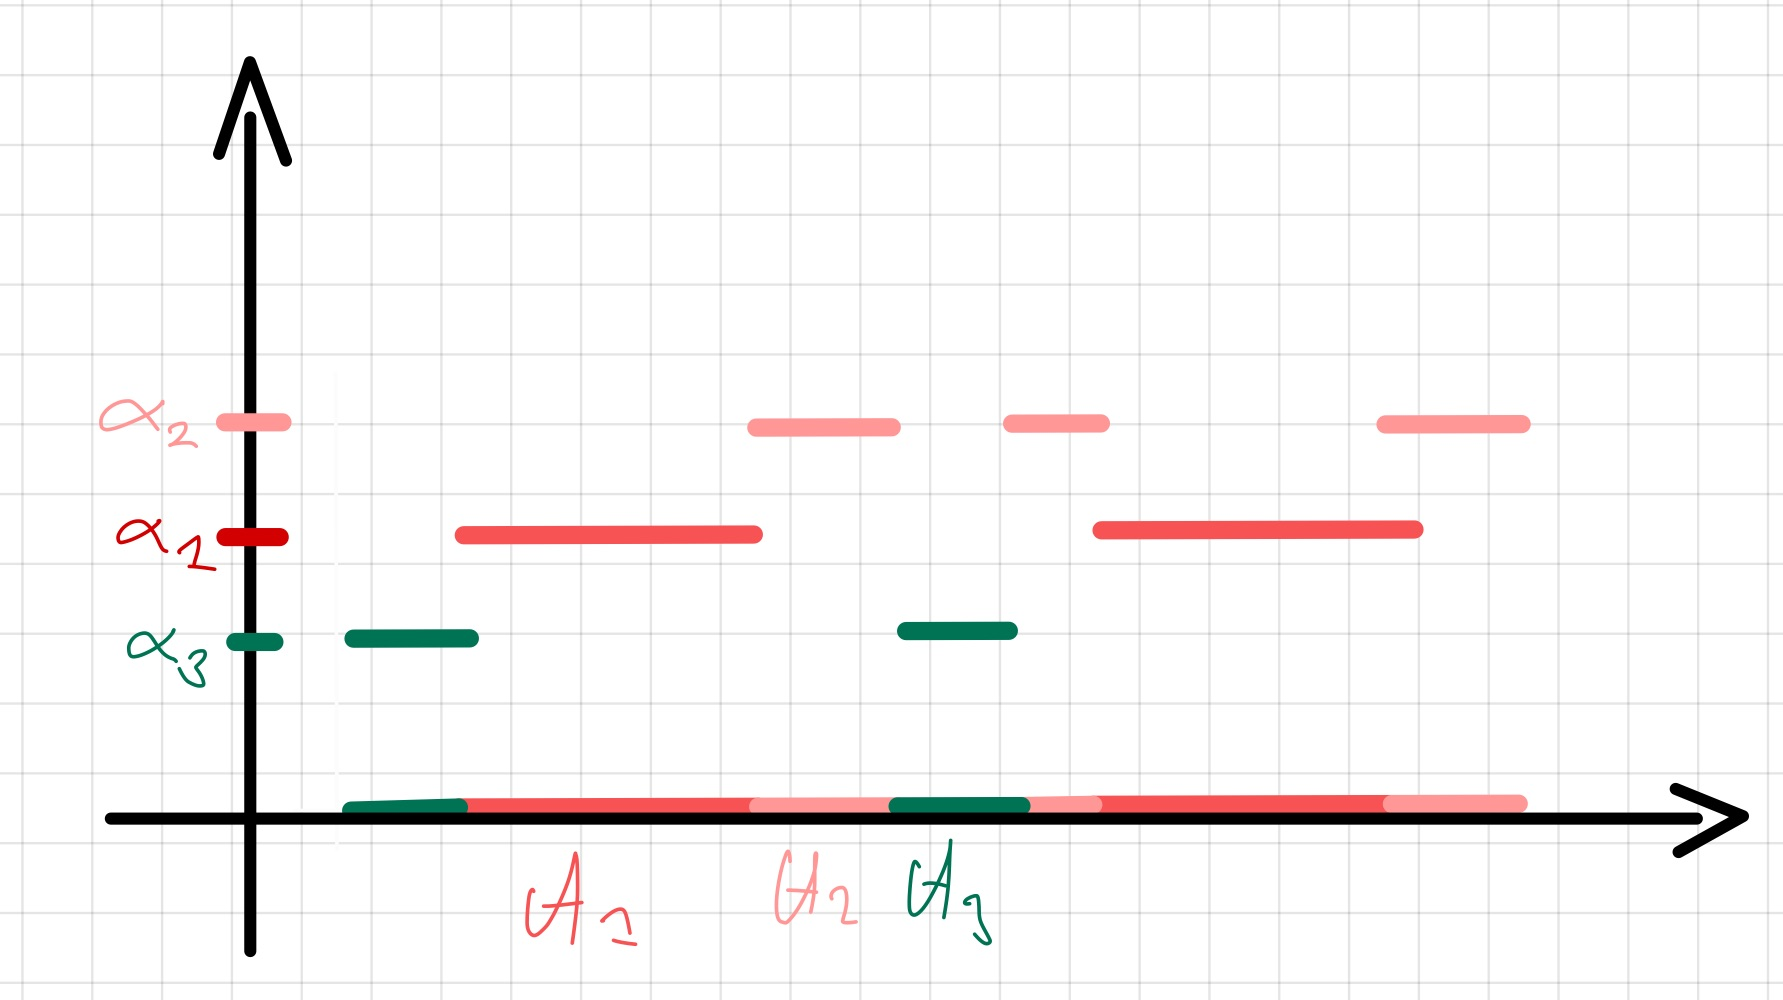
\includegraphics[width=\textwidth]{../\string_build/html/\string_images/simplefun.jpg}
\caption{Visualisierung einer einfachen Funktion.}\label{\detokenize{masstheorie/lebesgue_integral:fig-simplefun}}\end{figure}
\begin{definition}{}{masstheorie/lebesgue_integral:definition-7}



\par
Eine Funktion \(f:\R^n\to\overline{R}\) heißt einfach, falls Koeffizienten \(\alpha_i\in\overline{\R}\) und messbare Mengen \(A_i\in\mathcal{A}(\R^n)\) für \(i=1,\ldots,N\) existieren, s.d.,
\begin{align*}
f = \sum_{i=1}^N \alpha_i \bone_{A_i}.
\end{align*}\end{definition}

\par
Man erhält über die Definition direkt ein Lemma, dass einfache Funktionen Lebesgue messbar sind.
\begin{lemma}{}{masstheorie/lebesgue_integral:lemma-8}



\par
Es sei \(f:\R^n\to\overline{\R}\) eine einfache Funktion, dann ist \(f\) Lebesgue messbar.
\end{lemma}

\begin{proof}
 Siehe \href{https://www.fau.tv/clip/id/40589}{Vorlesung} ab Minute 8:45.
\end{proof}

\par
Für einfache Funktionen können wir analog zum Riemann Integral das Lebesgue Integral definieren, indem wir das Maß der einzelnen Mengen multipliziert mit den Funktionswerten summieren, welche eine einfache Funktion erzeugen.
\begin{remark}{(Wohldefiniertheit)}{masstheorie/lebesgue_integral:remark-9}



\par
Es ist wichtig anzumerken, dass für eine einfache Funktion \(f\) verschiedene Zerlegungen in Mengen \(A_i\) und Koeffizienten \(\alpha_i\) existieren. Allerdings erkennen wir, dass der Wert des Integrals unabhängig von der Wahl der Zerlegung ist und das Intergal somit wohldefiniert ist.
\end{remark}


\subsection{Das Lebesgue Integral nicht negativer Funktionen}
\label{\detokenize{masstheorie/lebesgue_integral:das-lebesgue-integral-nicht-negativer-funktionen}}
\par
Die wichtige Eigenschaft, welche die Betrachtung von einfachen Funktion so relevant macht, ist dass sich messbare Funktionen beliebig gut durch einfache Funktionen approximieren lassen. Diese Tatsache formulieren wir in folgendem Lemma.
\begin{lemma}{}{masstheorie/lebesgue_integral:lem:simplefun}



\par
Sei \(f \colon \Omega \to [0,\infty]\) eine Lebesgue messbare Funktion, dann existiert eine monoton wachsende Folge \((f_i)_{i_\in N}\) von einfachen Funktionen mit
\begin{align*}
f_i&\leq f_{i+1}\\
f_i &= 0\text{ in }\Omega^C\\
f&=\lim_{i\to\infty} f_i.
\end{align*}\end{lemma}

\begin{proof}
 Siehe \href{https://www.fau.tv/clip/id/40589}{Vorlesung} ab Minute 13:00.
\end{proof}

\par
Mithilfe der Tatsache, dass sich messbare Funktionen beliebig gut durch einfache Funktionen approximieren lassen, können wir nun das Lebesgue Integral für nicht negative messbare Funktionen einführen.
\begin{definition}{}{masstheorie/lebesgue_integral:definition-11}



\par
Es sei \(f:\Omega\to[0,\infty]\) Lebesgue messbar und nach \cref{masstheorie/lebesgue_integral:lem:simplefun} \((f_i)_{i\in\N}\) eine monoton wachsende Folge von einfachen Funktionen mit \(\lim_{i\to\infty} f_i = f\), dann ist das \textbf{Lebesgue Integral} von \(f\) definiert durch
\begin{align*}
\int_{\Omega} f \,d\lambda^n = \lim_{i\rightarrow \infty} \int_{\R^n} f_i \,d\lambda^n.
\end{align*}\end{definition}

\par
Wir zeigen im Folgenden wichtige Eigenschaften des Lebesgue Integrals.
\begin{theorem}{(Eigenschaften des Lebesgue Integrals)}{masstheorie/lebesgue_integral:theorem-12}



\par
Das Lebesgue Integral ist \emph{wohldefiniert}, d.h., sein Wert ist unabhängig von der gewählten Folge von einfachen Funktionen \((f_n)_{n\in\N}\).
Darüber hinaus ist das Lebesgue Integral \emph{linear} und \emph{monoton}, d.h., für nicht negative, Lebesgue messbare Funktionen \(f,g \geq 0,\alpha\in\overline{\R}\) gilt
\begin{align*}
\int_\Omega f+\alpha\,g\,d\lambda^n = \int_\Omega f\,d\lambda^n + \alpha\, \int_\Omega g d\lambda^n\\
f \leq g \quad \Rightarrow \quad \int_\Omega f\, d\lambda^n \leq \int_\Omega g\, d\lambda^n.
\end{align*}\end{theorem}

\begin{proof}
 Siehe \href{https://www.fau.tv/clip/id/40589}{Vorlesung} ab Minute 30:00.
\end{proof}

\par
Anstatt der Folge von einfachen Funktionen, kann man auch eine beliebige monotone Folge von messbaren Funktionen benutzen um das Integral zu approximieren. Diese Aussage ist unter dem \textbf{Satz von der monotonen Konvergenz} oder dem \textbf{Konvergenzsatz von Beppo Levi} bekannt.

\begin{emphBox}{Beppo Levi}{}

\par
\href{https://de.wikipedia.org/wiki/Beppo\_Levi}{Beppo Levi} (Geboren 14. Mai 1875 in Turin, Italien; Gestorben 28. August 1961 in Rosario, Argentinien) war ein italienischer Mathematiker.
\end{emphBox}
\begin{lemma}{}{masstheorie/lebesgue_integral:lem:levi}



\par
Es sei \(f_i:\R^n\to[0,\infty],i\in\N\) eine Folge nicht negativer Lebesgue messbarer Funktionen mit
\begin{align*}
f_i\leq f_{i+1}\qquad\text{(Monotonie))},\\
\lim_{i\to\infty} f_i = f\qquad\text{(Konvergenz)},
\end{align*}
\par
wobei \(f:[0,\infty]\to\overline{\R}\) auch Lebesgue messbar ist, dann gilt
\begin{align*}
\lim_{i\to\infty} \int_{\R^n} f_i \,d\lambda^n = \int_{\R^n} f \,d\lambda^n
\end{align*}\end{lemma}

\begin{proof}
 Ref missing.
\end{proof}

\par
Eine weitere Aussage in diesem Kontext ist das \textbf{Lemma von Fatou}, welches eine Abschätzung für eine nicht notwendigerweise konvergierende Folge von Funktionen zeigt.

\begin{emphBox}{Pierre Fatou}{}

\par
\href{https://de.wikipedia.org/wiki/Pierre\_Fatou}{Pierre Joseph Louis Fatou} (Geboren 28. Februar 1878 in Lorient; Gestorben 10. August 1929 in Pornichet) war ein französischer Mathematiker.
\end{emphBox}
\begin{lemma}{}{masstheorie/lebesgue_integral:lemma-14}



\par
Es sei \(f_i:\R^n\to[0,\infty],i\in\N\) eine Folge nicht negativer Lebesgue messbarer Funktion, dann ist
\begin{align*}
f(x) := \liminf_{i\to\infty} f_i(x)
\end{align*}
\par
nicht negativ und Lebesgue messbar und es gilt
\begin{align*}
\liminf_{i\to\infty} \int_{\R} f_i\, d\lambda^n \geq \int_\R^n f\, d\lambda^n.
\end{align*}\end{lemma}

\begin{proof}
 Ref missing.
\end{proof}


\subsection{Das Lebesgue Integral integrierbarer Funktionen}
\label{\detokenize{masstheorie/lebesgue_integral:das-lebesgue-integral-integrierbarer-funktionen}}
\par
Wir wollen nun das Lebesgue Integral auf messbaren Funktionen mit wechselndem Vorzeichen betrachten. Dafür spalten wir eine Funktionen in ihren positiven und ihren negativen Teil auf und bilden das Integral über diese Funktionen. Um die beiden Teile aufsummieren zu können, müssen wir allerdings fordern, dass beide endlich sind.
\begin{definition}{}{masstheorie/lebesgue_integral:definition-15}



\par
Sei \(f \colon \R^n \rightarrow \R\) eine Lebesgue messbare Funktion, wir nennen die Funktion \(f\) \textbf{Lebesgue integrierbar}, falls
\begin{align*}
\int_{\R^n} \abs{f} d\lambda^n < +\infty
\end{align*}
\par
gilt. Für eine Lebesgue integrierbare Funktion \(f\), definieren wir entsprechende positive integrierbare Funktionen
\begin{align*}
f^+ := \max \lbrace f, 0 \rbrace, \qquad f_- := \max{-f, 0},
\end{align*}
\par
so dass gilt \(f = f^+ - f_-\). Dann können wir das \textbf{Lebesgue Integral} von \(f\) definieren als
\begin{align*}
\int_{\R^n} f\, d\lambda^n := \int_{\R^n} f^+\, d\lambda^n - \int_{\R^n} f_-\, d\lambda^n.
\end{align*}\end{definition}
\begin{lemma}{}{masstheorie/lebesgue_integral:lemma-16}



\par
Das Lebesgue Integral ist ein linearer und monotoner Operator auf der Menge der Lebesgue integrierbaren Funktionen.
\end{lemma}

\begin{proof}
 ToDo
\end{proof}

\par
Auch für integrierbare Funktionen gibt es einen wichtigen Konvergenzsatz, der \textbf{Konvergenzsatz von Lebesgue} oder auch der \textbf{Satz von der dominierten Konvergenz}.
\begin{theorem}{}{masstheorie/lebesgue_integral:theorem-17}



\par
Es sei \(f_i:\R^n\to\R\) eine Folge Lebesgue messbarer Funktionen mit \(\lim_{i\to\infty} f_i =f\) und \(\abs{f}\leq g\) wobei \(g\) eine Lebesgue integrierbare Funktion ist, dann gilt \(f\) ist Lebesgue integrierbar und
\begin{align*}
\lim_{i\to\infty} \int_{\R^n} f_i\, d\lambda^n = \int_{\R^n} f\, d\lambda^n.
\end{align*}\end{theorem}

\begin{proof}
 Ref missing.
\end{proof}


\subsection{Fast überall Eigenschaften}
\begin{definition}{}{\detokenize{masstheorie/lebesgue_integral:fast-uberall-eigenschaften}}\label{masstheorie/lebesgue_integral:definition-18}



\par
Seien \(f,g \colon \R^n \rightarrow \overline{\R}\) Lebesgue messbare Funktionen.
Wir sagen \(f = g\) \textbf{fast sicher} bezüglich des Lebesgue Maßes genau dann, wenn eine Lebesgue Nullmenge \(N\) existiert, so dass gilt
\begin{align*}
f(x) = g(x) \quad \forall x \in \R^n \setminus N.
\end{align*}\end{definition}


\section{Integrationstechniken}
\label{\detokenize{masstheorie/integrationstechnik:integrationstechniken}}\label{\detokenize{masstheorie/integrationstechnik::doc}}
\par
In diesem Abschnitt beschäftigen wir uns mit Rechenmethoden und Rechenregeln, die es uns erlauben Funktionen mehrerer Variablen bezüglich des Lebesgue Maßes zu integrieren. Insbesondere lernen wir dadurch Verfahren kennen um Volumina und Flächen zu berechnen. Um diese Regeln formal zu zeigen benötigen wir zunächst etwas Theorie.


\subsection{Produktalgebren}
\label{\detokenize{masstheorie/integrationstechnik:produktalgebren}}
\par
Für zwei Messräume \((\Omega_1,\Sigma_1), (\Omega_2,\Sigma_2)\) wollen wir nun einen Produktraum erhalten. Hierbei werden wir auf Konzepte des \textbf{Tensorproduktes} zurückgreifen und benutzen deshalb die gleiche Notation. Wir definieren dann die Produkt \(\sigma\) Algebra,
\begin{align*}
\Sigma_1\otimes\Sigma_2 := \sigma\left(\Sigma_1\times\Sigma_2\right),
\end{align*}
\par
wobei
\begin{align*}
\Sigma_1\times\Sigma_2 = \left\{A_1\times A_2: A_1\in\Sigma_1, A_2\in\Sigma_2\right\}.
\end{align*}
\par
Wir arbeiten nicht auf Vektorräumen darum konstruieren wir \textbf{kein} Tensorprodukt im Sinnen von \hyperref[\detokenize{vektoranalysis/tensor:s-tensoren}]{Abschnitt \ref{\detokenize{vektoranalysis/tensor:s-tensoren}}}, aber die grundlegenden Konzepte sind ähnlich, weshalb es üblich ist, hier diese Notation zu verwenden. Weiterhin erkennen wir, dass mit dieser Konstruktion \(\Sigma_1\otimes\Sigma_2 \) eine \(\sigma\) Algebra auf \(\Omega_1\times\Omega_2\) ist.

\begin{figure}[htbp]
\centering


\noindent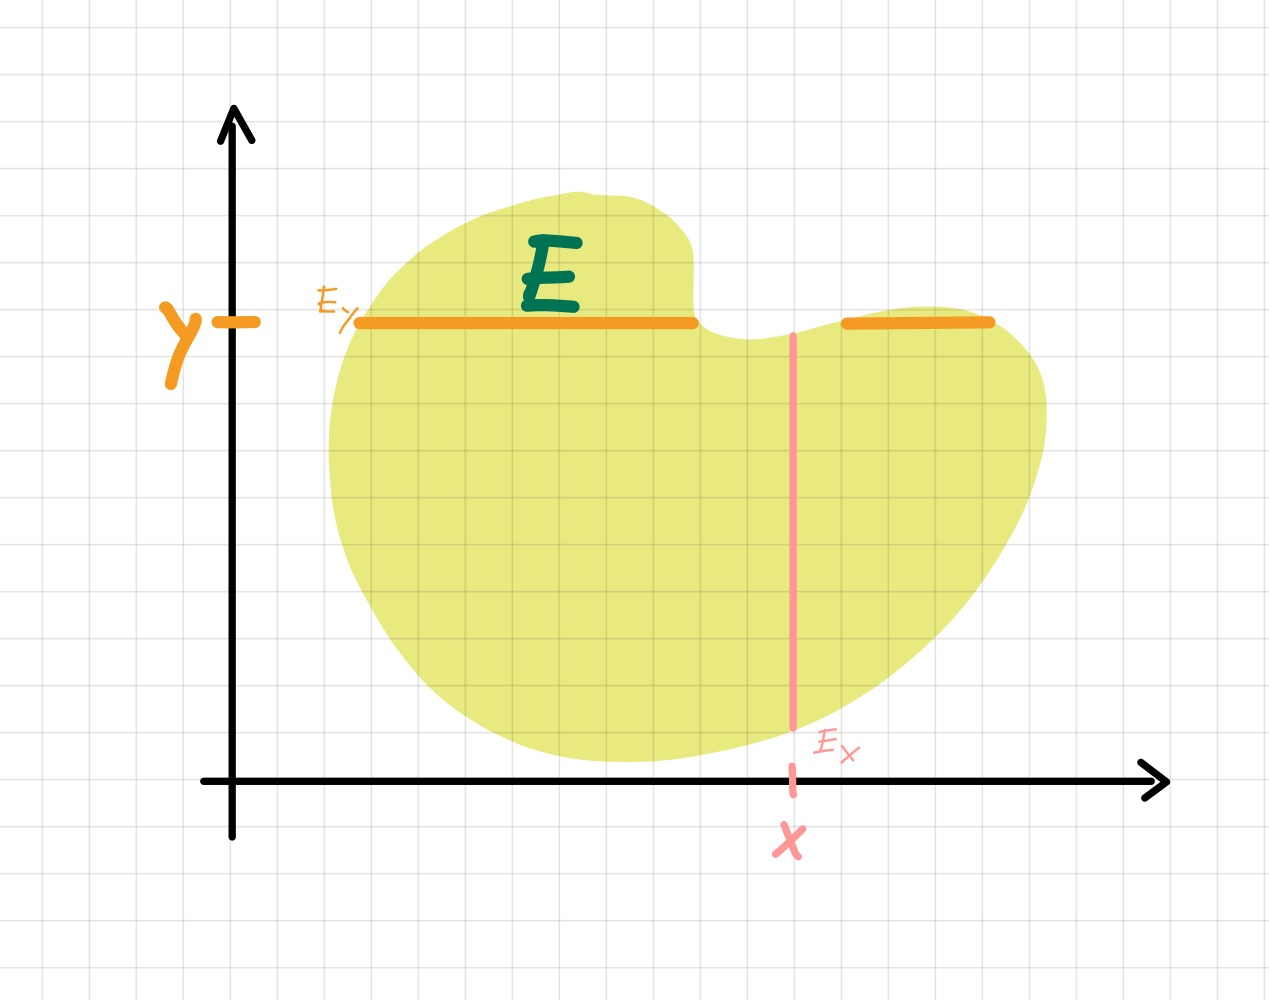
\includegraphics[width=\textwidth]{../\string_build/html/\string_images/schnitte.jpg}
\caption{Visualisierung von Mengenschnitten.}\label{\detokenize{masstheorie/integrationstechnik:fig-schnitte}}\end{figure}

\par
Für eine Menge \(E\subset\Omega_1\times\Omega_2\) betrachtet man in diesem Kontext oft sogenannte \textbf{Schnitte}
\begin{align*}
E_x := \{y\in \Omega_2: (x,y)\in E\}\subset\Omega_2\\
E^y := \{x\in \Omega_1: (x,y)\in E\}\subset\Omega_1
\end{align*}
\par
wofür man folgende Aussage hat.
\begin{lemma}{}{masstheorie/integrationstechnik:lem:secmeasure}



\par
Es seien \((\Omega_1,\Sigma_1), (\Omega_2,\Sigma_2)\) Messräume, dann gilt für eine Produktmessbare Menge \(E\in \Sigma_1\otimes\Sigma_2\), dass \(E_x\in \Sigma_2, E_y\in\Sigma_1\) für alle \(x\in\Omega_1,y\in\Omega_2\).
\end{lemma}

\begin{proof}
 Wir betrachten das Teilmengensystem
\begin{align*}
\M = \{E\subset\Omega_1\times\Omega_2:  E_x\in\Sigma_2, E^y\in\Sigma_1,\quad\forall x\in\Omega_1,  y\in\Omega_2\}
\end{align*}
\par
d.h. alle Mengen, welche die gewünschte Bedingung erfüllen. Wir sehen, dass für \(A\in\Sigma1,B\in\Sigma_2\) gilt
\begin{align*}
(A\times B)_x = 
\begin{cases}
B &\text{ falls }x\in A\\
\emptyset &\text{ sonst}
\end{cases}
\end{align*}
\par
und daher \((A\times B)_x\in\Sigma_2\) für alle \(x\in\Omega_1\). Analog zeigt man \((A\times B)^y\in\Sigma_1\) für alle \(y\in\Omega_2\) und daher gilt
\begin{align*}
\Sigma_1\times\Sigma_2\subset \M.
\end{align*}
\par
Weiterhin ist \(\M\) eine \(\sigma\) Algebra. Es gilt \(\emptyset\M\), weiterhin \((E^C)_x = (E_x)^C\)und analog \((E^C)^y= (E^y)^C\) und daher
gilt
\begin{align*}
E\in\M\Rightarrow E^C\in\M.
\end{align*}
\par
Weiterhin gilt für eine Folge von Mengen \(E_i\in\M,i\in\N\)
\begin{align*}
\left(\bigcup_{i\in\N} E_i\right)_x = \bigcup_{i\in\N} (E_i)_x
\end{align*}
\par
analog für den anderen Schnitt und daher
\begin{align*}
\bigcup_{i\in\N} E_i\in\M.
\end{align*}
\par
Somit folgt
\begin{align*}
\Sigma_1\otimes\Sigma_2=\sigma(\Sigma_1\times\Sigma_2)\subset \sigma(\M) = \M.
\end{align*}\end{proof}

\par
Speziell für \(\Omega_1=\R^n, \Omega_1=\R^m\) könnte man sich nun fragen wie sich die Produkt Algebra für die bekannten Borel und Lebesgue Algebren verhält. Zumindest für die Borel \(\sigma\) Algebra haben wir folgende Aussage.
\begin{lemma}{}{masstheorie/integrationstechnik:lemma-1}



\par
Für \(n,m\in\N\) gilt
\begin{align*}
\B(\R^n)\otimes \B(\R^m) = \B(\R^{n+m}).
\end{align*}\end{lemma}

\begin{proof}
 Offensichtlich gilt für den Mengen Ring
\begin{align*}
\mathcal{R}(\R^{n+m})=\left\{\bigcup_{i=1}^N Q_i: Q_i\subset\R^{n+m}\text{ ist halboffener Quader} \right\},
\end{align*}
\par
dass
\begin{align*}
\mathcal{R}(\R^{n+m})\subset \B(\R^n)\otimes \B(\R^m).
\end{align*}
\par
Weiterhin wissen wir aber auch nach \cref{masstheorie/masstheorie:s-gentop} , dass \(\sigma(\mathcal{R}(\R^{n+m})) = \B(\R^{n+m})\) und somit
\begin{align*}
\B(\R^{n+m})\subset \B(\R^n)\otimes \B(\R^m).
\end{align*}
\par
Für die andere Richtung sei \(A_1\in\B(\R^n) A_2\in\B(\R^m)\), dann gilt
\begin{align*}
A_1\times A_2 = \left(A_1\times\R^m\right) \cap (\R^n\times A_2) =\pi_1^{-1}(A_1) \cap \pi_2^{-1}(A_2)
\end{align*}
\par
wobei \(\pi_1:\R^{n+m}\to\R^n,\pi_2:\R^{n+m}\to\R^m\) die Projektionen
\begin{align*}
\pi_1(z_1,\ldots,z_{n+m})&= (z_1,\ldots, z_n)\\
\pi_2(z_1,\ldots,z_{n+m})&= (z_{n+1},\ldots, z_{n+m})
\end{align*}
\par
sind. Da Projektionen stetig sind, sind sie Borel messbar nach ?? und daher gilt
\begin{align*}
\pi_1^{-1}(A_1)\in B(\R^{n+m})\\
\pi_2^{-1}(A_2)\in B(\R^{n+m}).
\end{align*}
\par
Daraus folgern wir, dass
\begin{align*}
A_1\times A_2 \in \B(\R^{n+m})
\end{align*}
\par
und somit
\begin{align*}
\B(\R^n)\otimes \B(\R^m)\subset\B(\R^{n+m}).
\end{align*}\end{proof}

\par
Für die Lebesgue \(\sigma\) Algebren gilt diese Identität nicht, allgemein kann man zeigen, dass
\begin{align*}
\mathcal{A}(\R^n)\otimes\mathcal{A}(\R^m)\subset \mathcal{A}(\R^{n+m})
\end{align*}
\par
allerdings ist die Menge auf der rechten Seite echt größer wie das folgende Beispiel zeigt.
\begin{example}{}{masstheorie/integrationstechnik:ex:prodsig}



\par
Wir betrachten die zwei Lebesgue Algebren für \(n=m=1\), dh. \(\mathcal{A}(\R)\). Nach \hyperref[\detokenize{masstheorie/masstheorie:s-vitali}]{Abschnitt \ref{\detokenize{masstheorie/masstheorie:s-vitali}}} gibt es Mengen \(V\subset\R\) sogenannte Vitali Mengen s.d. \(V\not\in\mathcal{A}(\R)\). Weiterhin erkennen wir, dass für das Lebesgue Maß auf \(\R^2\) folgt, dass
\begin{align*}
\lambda^{2}(V\times\{0\}) = 0
\end{align*}
\par
dies folgt mit der Argumentation aus Aufgabe??. Daher ist \(V\times\{0\}\in \mathcal{A}(\R^2)\) da es eine Nullmenge ist.

\par
Wir erkennen aber, dass sich \(V\) als Schnitt dieser Produkt Menge darstellen lässt, nämlich
\begin{align*}
V = (V\times\{0\})^0
\end{align*}
\par
wäre nun \((V\times\{0\})^0\in \mathcal{A}(\R)\otimes\mathcal{A}(\R)\) so würde mit \cref{masstheorie/integrationstechnik:lem:secmeasure} folgen, dass auch der Schnitt \(V\in\mathcal{A}(\R)\) gilt, was ein Widerspruch ist, daher
\begin{align*}
(V\times\{0\})^0 \not\in  \mathcal{A}(\R)\otimes\mathcal{A}(\R).
\end{align*}\end{example}

\par
Das abstrakte Konzept, welches sich hinter diesem Beispiel verbirgt wir mit dem Begriff Vollständigkeit eines Maßes bezeichnet.
\begin{definition}{}{masstheorie/integrationstechnik:definition-3}



\par
Ein Maßraum \((\Omega,\Sigma,\mu)\), falls für jede \(\mu\) Nullmenge \(N\in\Sigma, \mu(N)=0\) gilt
\begin{align*}
A\subset N \Rightarrow A\in \Sigma.
\end{align*}\end{definition}
\begin{remark}{}{masstheorie/integrationstechnik:remark-4}



\par
Wir wissen, dass jede Menge die bezüglich des äußeren Maßes \(\lambda^\ast\) eine Nullmenge ist auch Lebesgue messbar ist. Daher ist das Lebesgue Maß ein vollständiges Maß.
\end{remark}

\par
Weiterhin lässt sich ein beliebiges Maß vervollständigen, indem wir die \(\sigma\) Algebra
\begin{align*}
\overline{\Sigma}:=\{A\cup N: A\in\Sigma, N\subset B\in\Sigma\text{ mit }\mu(B)=0\}
\end{align*}
\par
betrachten zusammen mit dem Maß
\begin{align*}
\overline{\mu}(B)= \overline{\mu}(A\cup N):= \mu(A).
\end{align*}
\par
Hier lässt sich nun folgendes zeigen.
\begin{lemma}{}{masstheorie/integrationstechnik:lem:completelebesgue}



\par
Für \(n,m\in\N\) gilt
\begin{align*}
\overline{\mathcal{A}(\R^n)\otimes\mathcal{A}(\R^m)}= \mathcal{A}(\R^{n+m}).
\end{align*}\end{lemma}

\begin{proof}
 Siehe z.B. \cite{Bog07} Theorem 1.5.6.
\end{proof}


\subsection{Produktmaße}
\label{\detokenize{masstheorie/integrationstechnik:produktmasze}}
\par
Wir wollen nun Maße auf der Produktalgebra betrachten.
\begin{definition}{}{masstheorie/integrationstechnik:definition-6}



\par
Es seien \((\Omega_1,\Sigma_1,\mu_1), (\Omega_2,\Sigma_2,\mu_2)\) zwei Maßräume, dann heißt ein Maß \(\mu\) auf dem Messraum \((\Sigma_1\otimes\Sigma_2, \Omega_1\times\Omega_2)\) \textbf{Produktmaß}, falls
\begin{align*}
\mu(A_1\times A_2) = \mu_1(A_1)\cdot\mu_2(A_2)\quad\forall A_1\in\Sigma_1, A_2\in\Sigma_2.
\end{align*}\end{definition}
\begin{remark}{}{masstheorie/integrationstechnik:remark-7}



\par
In \cref{vektoranalysis/tensor:s-grass}  haben wir das Tensorprodukt zweier lineare Abbildungen \(T_1,T_2\) definiert über
\begin{align*}
(T_1\otimes T_2)(v_1,V_2) := T_1(v_1)\cdot T_2(v_2).
\end{align*}
\par
Es sei hier erwähnt, dass das Maß \textbf{keine} lineare Abbildung ist, insbesondere haben wir keinen Vektorraum gegeben. Die Produktstruktur ist trotzdem ähnlich, weshalb eine gewisse Analogie zwischen dem Tensorprodukt und dem Produktmaß herrscht.
\end{remark}
\begin{remark}{}{masstheorie/integrationstechnik:remark-8}



\par
In den obigen Produkten können einzelnen Terme jeweils unendlich werden, hierbei benutzt man die Konvention
\begin{align*}
0 * a = 0\quad\forall a\in\overline{\R}.
\end{align*}\end{remark}

\par
Man kann zeigen, dass ein Produktmaß stets existiert siehe ??. Allerdings ist es nicht notwendigerweise eindeutig bestimmt, hierfür benötigt man die sogennate \(\sigma\) Endlichkeit.
\begin{definition}{}{masstheorie/integrationstechnik:definition-9}



\par
Es sei \((\Omega,\Sigma,\mu)\) ein Maßraum, das Maß \(\mu\) heißt \(\sigma\)\textbf{ endlich}, falls eine Folge von Mengen \(A_i\in\Sigma,i\in\N\) existiert, s.d., \(\mu(A_i)<\infty\) und
\begin{align*}
\bigcup_{i\in\N} A_i = \Omega.
\end{align*}\end{definition}
\begin{remark}{}{masstheorie/integrationstechnik:remark-10}



\par
Das wichtigste Beispiel für uns ist das Lebesgue Maß auf \(\R^n\) welches bezüglich der Borelschen \(\sigma\) Algebra zwar nicht endlich aber \(\sigma\) endlich ist. Insbesondere ist es damit auch \(\sigma\) endlich bezüglich der Lebesgue \(\sigma\) Algebra \(\mathcal{A}\).
\end{remark}

\par
Für \(\sigma\) endliche Maße kann man zeigen, dass ein eindeutig bestimmtes Produktmaß existiert.
\begin{theorem}{}{masstheorie/integrationstechnik:theorem-11}



\par
Es seien \((\Omega_1,\Sigma_1,\mu_1), (\Omega_2,\Sigma_2,\mu_2)\) zwei \(\sigma\) endliche Maßräume, dann existiert eine eindeutig bestimmtes Produktmaß
\begin{align*}
\mu_1\otimes \mu_2:\Sigma_1\otimes\Sigma_2\to[0,\infty],
\end{align*}
\par
s.d. die Bedingung
\begin{align*}
(\mu_1\otimes\mu_2)(A\times B) = \mu_1(A)\cdot\mu_2(B)\quad\forall A\in\Sigma_1, B\in\Sigma_2,
\end{align*}
\par
erfüllt ist.
\end{theorem}

\begin{proof}
 See Bogachev ref missing.
\end{proof}

\par
Anhand von \cref{masstheorie/integrationstechnik:ex:prodsig} haben wir gesehen, dass die Lebesgue \(\sigma\) Algebra auf \(\R^{n+m}\) größer ist als die Produkt \(\sigma\) Algebra. Allerdings kann man zeigen, dass das Produktmaß zumindest auf der kleineren Produktalgebra übereinstimmt.
\begin{lemma}{}{masstheorie/integrationstechnik:lem:lebesguecomp}



\par
Es gilt
\begin{align*}
\lambda^{n+m} = \overline{\lambda^n\otimes\lambda^m},
\end{align*}
\par
insbesondere folgt damit für eine beliebige Menge \(E\in \mathcal{A}(\R^n)\otimes\mathcal{A}(\R^m)\)
\begin{align*}
\lambda^{n+m}(E) = (\lambda^n\otimes\lambda^m)(E).
\end{align*}\end{lemma}

\begin{proof}
 Siehe z.B. \cite{Bog07} Theorem 1.5.6.
\end{proof}

\par
Speziell für \(A_1\in\mathcal{A}(\R^n), A_2\in\mathcal{A}(\R^m)\) folgt damit
\begin{align*}
\lambda^{n+m}(A^1\times A^2)=\lambda^{n}(A^1)\cdot\lambda^{m}(A^2).
\end{align*}

\subsection{Das Prinzip von Cavalieri}
\label{\detokenize{masstheorie/integrationstechnik:das-prinzip-von-cavalieri}}
\par
Im vorherigen Abschnitt haben wir Produkte von Maßen betrachtet. Insbesondere haben wir erkannt, dass wir für Mengen der Form \(A\times B\), dass Lebesgue Maß multiplikativ aufteilen können,
\begin{align*}
\lambda^{n+m}(A\times B) = \lambda^n(A)\,\lambda^m(B).
\end{align*}
\par
Unser Ziel ist es nun das Lebesgue Maß beliebige messbare Mengen \(E\subset\R^{n+m}\) mithilfe der niedrigdimesnionaleren Lebesgue Maße auszudrücken. Dies führt auf das sogenannte Prinzip von Cavalieri.

\begin{emphBox}{Bonaventura Cavalieri}{}

\par
\href{https://de.wikipedia.org/wiki/Bonaventura\_Cavalieri}{Bonaventura Francesco Cavalieri} (Geboren 1598 wahrscheinlich in Mailand; Gestorben 3. Dezember oder 30. November 1647 in Bologna; mit Gelehrtennamen Cavalerius) war ein italienischer Jesuat, Mathematiker und Astronom.
\end{emphBox}

\begin{figure}[htbp]
\centering


\noindent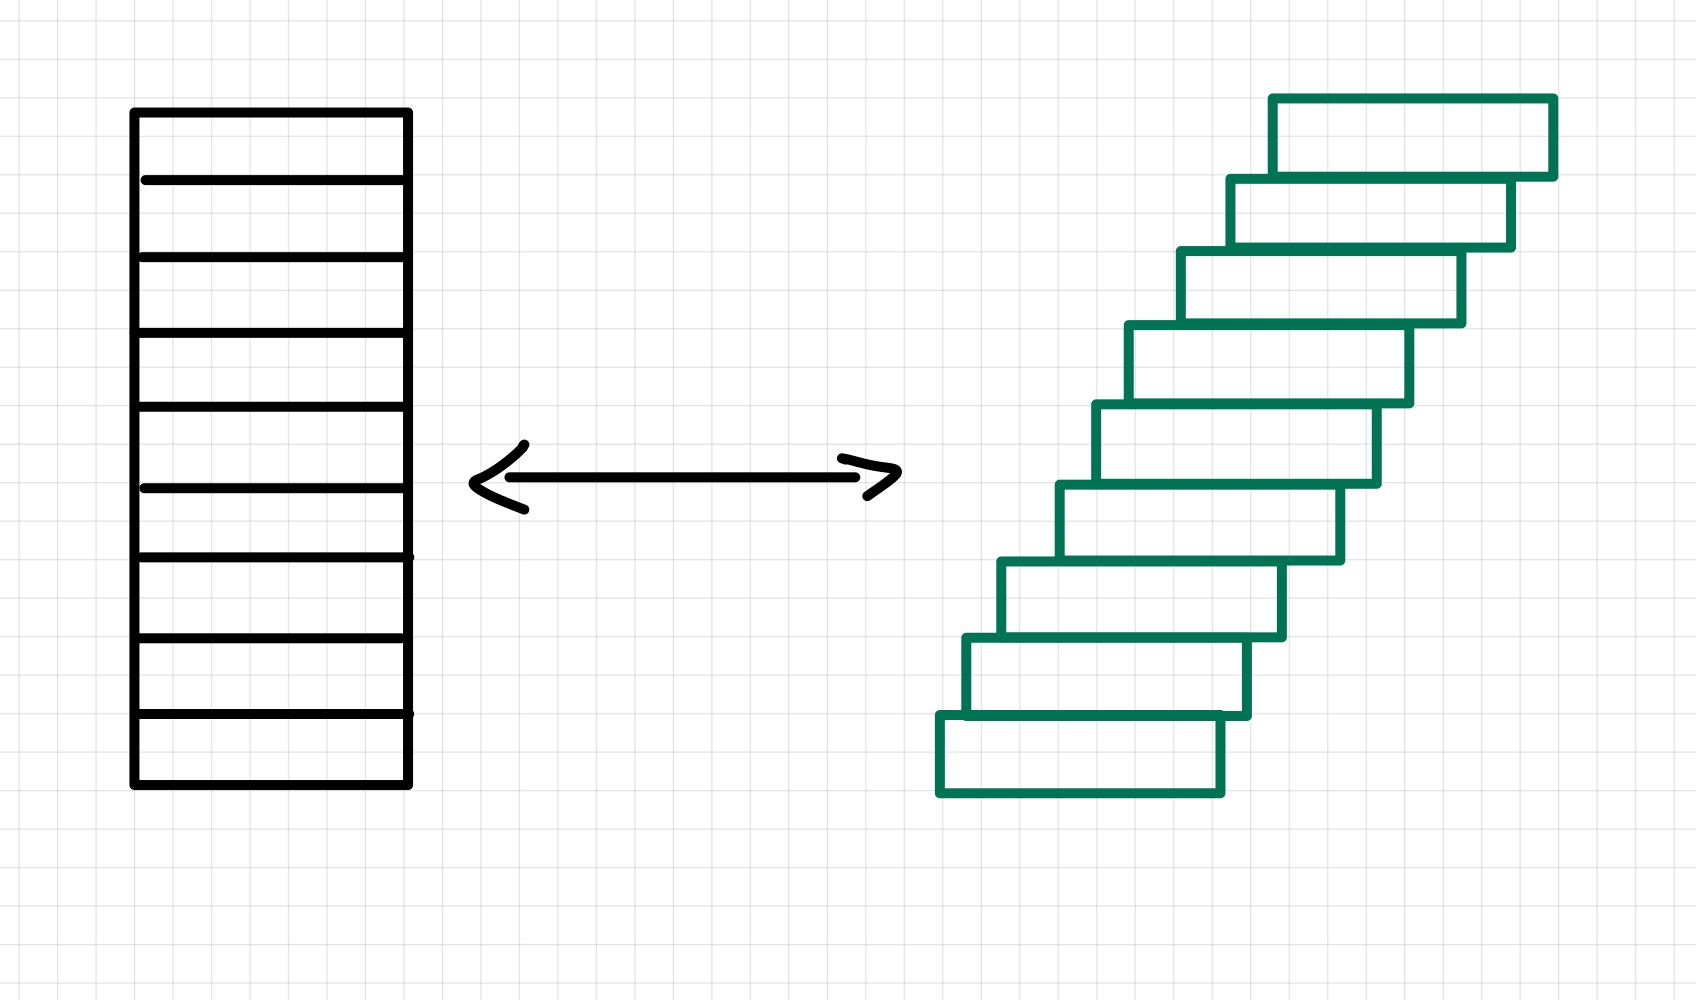
\includegraphics[width=\textwidth]{../\string_build/html/\string_images/cavalieri.jpg}
\caption{Visualisierung für das Prinzip von Cavalieri, beide Objekte haben die gleiche Fläche.}\label{\detokenize{masstheorie/integrationstechnik:fig-cavalieri}}\end{figure}

\par
Das Prinzip beruht auf der Intuition, dass zwei Körper, das gleiche Volumen haben, sofern alle ihre Schnittflächen welche parallel zu einer Grundfläche verlaufen gleich sind. Für \(\R^2\) ist dieses Prinzip in \hyperref[\detokenize{masstheorie/integrationstechnik:fig-cavalieri}]{Abb.\@ \ref{\detokenize{masstheorie/integrationstechnik:fig-cavalieri}}} dargestellt. Formal bedeutet das, dass wir für eine messbare Menge \(E\), den Inhalt über das Integral der Schnitte ausdrücken wollen, es gibt hier also drei Größen
\begin{align*}
\lambda^{n+m}(E), \int_{\R^n} \lambda^m(E_x) d\lambda^n(x), \int_{\R^m} \lambda^m(E_y) d\lambda^m(y)
\end{align*}
\par
welche wir in Beziehung zueinander setzten wollen.

\par
Ein Konzept was man in diesem Kontext benötigt, sind sogenannte monotone Klassen.
\begin{definition}{}{masstheorie/integrationstechnik:definition-13}



\par
Es sei \(\Omega\) eine Menge, ein Teilmengensystem \(\mathcal{C}\subset 2^\Omega\) heißt \textbf{monotone Klasse}, falls

\par
1. Für eine aufsteigende Folge von Mengen \(A_i\in\mathcal{C}, A_i\subset A_{i+1}, i\in\N\) gilt auch
\begin{align*}
\bigcup_{i\in\N} A_i\in\mathcal{C}.
\end{align*}
\par
1. Für eine absteigende Folge von Mengen \(A_i\in\mathcal{C}, A_i\supset A_{i+1}, i\in\N\) gilt auch
\begin{align*}
\bigcap_{i\in\N} A_i\in\mathcal{C}.
\end{align*}\end{definition}

\par
Offensichtlich ist jede \(\sigma\) Algebra eine monotone Klasse,die Umkehrung dieser Aussage gilt nicht im Allgemeinen.
Weiterhin arbeiten wir in diesem Kontext zusätzlich mit Mengenalgebren anstatt nur mit Mengenringen.
\begin{definition}{}{masstheorie/integrationstechnik:definition-14}



\par
Es sei \(\mathcal{R}\) ein Mengenring über der Menge \(\Omega\), gilt auch \(\Omega\in\mathcal{R}\), dann nennen wir \(\mathcal{R}\) \textbf{Mengenalgebra}.
\end{definition}
\begin{remark}{}{masstheorie/integrationstechnik:remark-15}



\par
Für zwei \(\sigma\) Algebren ist das kartesische Produkt \(\Sigma_1\times\Sigma_2\) i.A. keine Mengenalgebra, die Menge
\begin{align*}
\Sigma_1\diamond\Sigma_2:= \left\{\bigcup_{i=1}^N A^1_i\times A^2_i: A^1_i\in\Sigma_1, A^2_i\in\Sigma_2\quad i=1,\ldots,n\right\}
\end{align*}
\par
allerdings schon und sie erzeugt offensichtlich auch die Produkt \(\sigma\) Algebra,
\begin{align*}
\sigma(\Sigma_1\diamond\Sigma_2) = \Sigma_1\otimes\Sigma_2.
\end{align*}\end{remark}

\par
Betrachtet man analog zur kleinsten von \(\mathcal{C}\) erzeugten \(\sigma\) Algebra die kleinste von \(\mathcal{C}\) erzeugt monotone Klasse \(\text{M}\big[\mathcal{C}\big]\) so gilt folgendes hilfreiches Lemma.
\begin{lemma}{}{masstheorie/integrationstechnik:lem:monclass}



\par
Es sei \(\mathcal{C}\) eine Mengenalgebra, dann gilt
\begin{align*}
\sigma(\mathcal{C}) = \text{M}\big[\mathcal{C}\big].
\end{align*}\end{lemma}

\begin{proof}
 Siehe z.B. \cite{Tao07} Lemma 1.7.14.
\end{proof}

\par
Mithilfe des monotone Klassen Lemmas und den vorherigen Überlegungen können wir nun das Prinzip von Cavalieri beweisen.
\begin{theorem}{}{masstheorie/integrationstechnik:thm:cavalieri}



\par
Sei \(E \in \mathcal{A}(\R^n)\otimes\mathcal{A}(\R^m)\) mit \(\lambda^{n}\otimes\lambda^{m}(E) < \infty\),
dann gilt für fast alle \(x\in\R^n,y\in\R^m\), dass die Schnitte \(E_x, E^y\) auch Lebesgue messbar sind, die Funktionen
\begin{align*}
x \mapsto \lambda^m(E_x)\\
y \mapsto \lambda^n(E^y)
\end{align*}
\par
sind messbar und es gilt
\begin{align*}
\lambda^{n}\otimes\lambda^{m}(E) &= \int_{\R^n} \lambda^m(E_x) d\lambda^n(x)\\
&=
\int_{\R^m} \lambda^n(E^y) d\lambda^m(y).
\end{align*}\end{theorem}

\begin{proof}
 Es sei \(\mathcal{C}\subset\mathcal{A}(\R^n)\otimes\mathcal{A}(\R^m)\) das System aller Mengen s.d. die Aussage gilt. Dann ist \(\mathcal{C}\) eine monotone Klasse und
\begin{align*}
\mathcal{A}(\R^n)\diamond\mathcal{A}(\R^m)\subset \mathcal{C}.
\end{align*}
\par
Mit dem monotone Klassen Lemma (\cref{masstheorie/integrationstechnik:lem:monclass}  folgt dann
\begin{align*}
\mathcal{A}(\R^n)\otimes\mathcal{A}(\R^m) = \sigma(\mathcal{A}(\R^n)\diamond\mathcal{A}(\R^m)) = 
\text{M}\big[\mathcal{A}(\R^n)\diamond\mathcal{A}(\R^m)\big] \subset 
\text{M}\big[\mathcal{C}\big] = \mathcal{C}.
\end{align*}\end{proof}

\par
Ein Korollar aus der obigen Aussage ist, dass fast alle Schnitte einer \(\lambda^n\otimes\lambda^m\) Nullmenge selbst Nullmengen bezüglich \(\lambda^n\), bzw. \(\lambda^m\) sind.
\label{masstheorie/integrationstechnik:cor:zeroprodset}
\begin{emphBox}{}{}{Corollary 5.2}



\par
Es sei \(E\in\mathcal{A}(\R^n)\otimes\mathcal{A}(\R^m)\) eine Nullmenge, dann folgt, dass für fast alle \(x\in\R^n,y\in\R^m\) auch \(\lambda^m(E_x)=0=\lambda^n(E^y)\) gilt.
\end{emphBox}

\begin{proof}
 Für die Funktion \(f:x\mapsto \lambda^m(E_x)\) gilt mit dem Prinzip von Cavalieri, dass
\begin{align*}
0 = \lambda^{n}\otimes\lambda^{m}(E) = \int_{\R^n} f(x)d\lambda^n(x)
\end{align*}
\par
und daher mit ??, dass
\begin{align*}
f(x)=\lambda^m(E_x)=0
\end{align*}
\par
für fast alle \(x\in\R^n\). Die Aussage für \(\lambda^n(E^y)\) folgt analog.
\end{proof}

\par
Diese Korollar erlaubt es uns die Aussage von Cavalieri auf alle Mengen \(E\in \mathcal{A}(\R^{n+m})\) zu verallgemeinern.
\begin{lemma}{}{masstheorie/integrationstechnik:lemma-19}



\par
Die Aussage von \cref{masstheorie/integrationstechnik:thm:cavalieri} gilt auch für Mengen \(E\in \mathcal{A}(\R^{n+m})\).
\end{lemma}

\begin{proof}
 Es sei \(E\in \mathcal{A}(\R^{n+m})\), nach \cref{masstheorie/integrationstechnik:lem:completelebesgue} existieren Mengen \(\tilde{E}\in\mathcal{A}(\R^n)\otimes\mathcal{A}(\R^m)\), \(N\subset \tilde{N}\), s.d.
\begin{align*}
E = \tilde{E}\cup N\\
(\lambda^n\otimes\lambda^m)(\tilde{N}) = 0.
\end{align*}
\par
Insbesondere ist dann
\begin{align*}
E\setminus \tilde{N} = \left(\tilde{E}\setminus \tilde{N} \right)\cup \underbrace{\left(N\setminus \tilde{N}\right)}_{=\emptyset} = 
\tilde{E}\setminus \tilde{N}\in \in\mathcal{A}(\R^n)\otimes\mathcal{A}(\R^m)
\end{align*}
\par
daher können wir \cref{masstheorie/integrationstechnik:thm:cavalieri} auf \(E\setminus \tilde{N}\) anwenden. Da aber fast alle Schnitte \(\tilde{N}_x,\tilde{N}^y\) Nullmengen sind, gilt die Aussage, dann für fast alle \(x,y\in E\).
\end{proof}

\par
Mit dieser Aussage können wir nun ein Beispiel betrachten, in welchem wir die Fläche eines Kreises berechnen.

\begin{figure}[htbp]
\centering


\noindent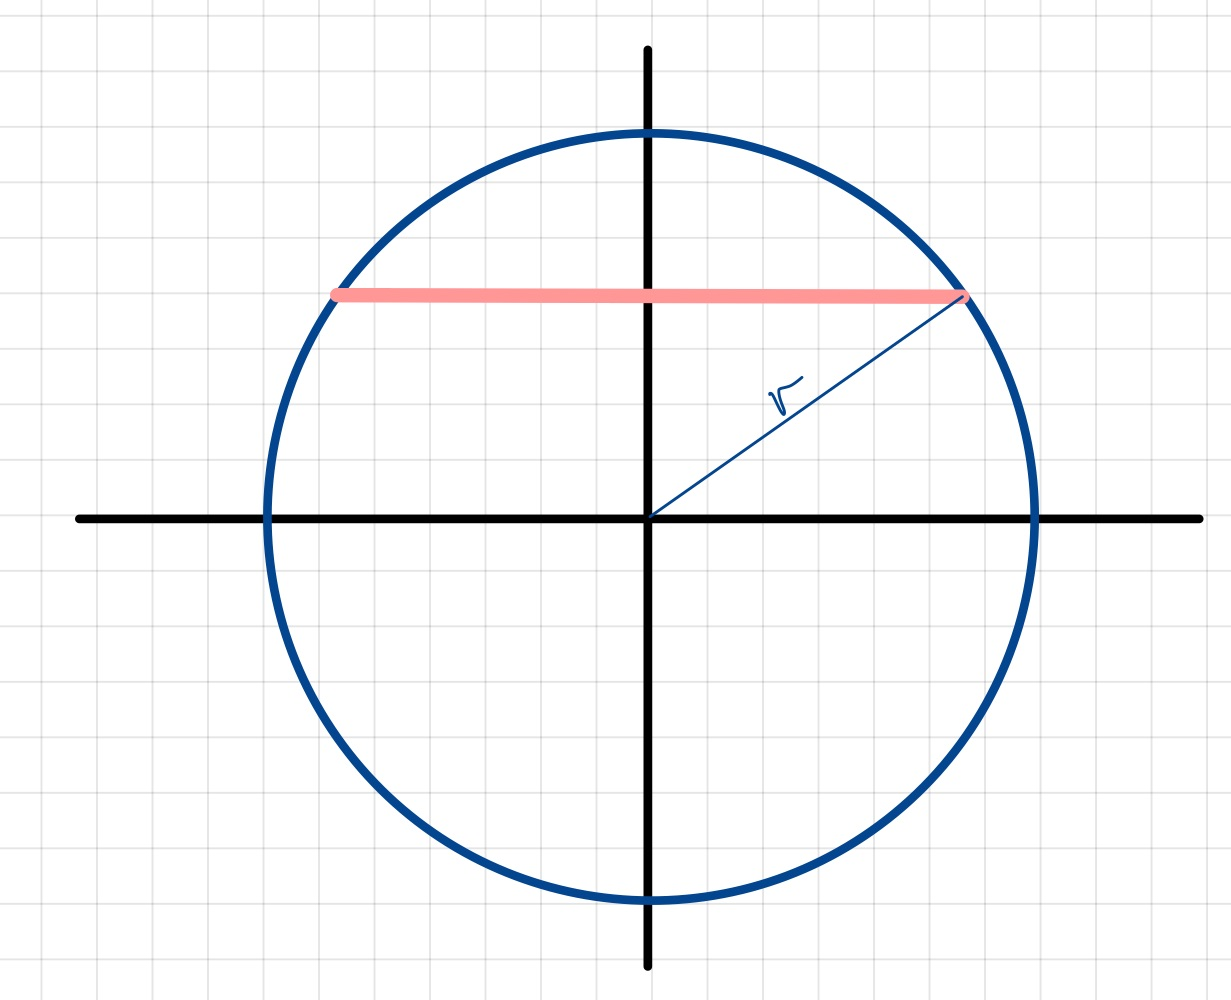
\includegraphics[width=\textwidth]{../\string_build/html/\string_images/ball.jpg}
\caption{Visualisierung für \cref{masstheorie/integrationstechnik:ex:ball} }\label{\detokenize{masstheorie/integrationstechnik:fig-ball}}\end{figure}
\begin{example}{}{masstheorie/integrationstechnik:ex:ball}



\par
Wir betrachten den \(2\) dimensionale Ball
\begin{align*}
B_r^2:=\{x\in\R^2: |x|\leq r\},
\end{align*}
\par
wir erkennen, dass sich ein Schnitt für \(\abs{y}\leq r\) jeweils ergibt durch
\begin{align*}
(B_r^2)_y = \{x:(x,y)\in B_r^2\} = \{x\leq\sqrt{r^2-y^2}\} = [-\sqrt{r^2-y^2},\sqrt{r^2-y^2}]
\end{align*}
\par
und ansonsten leer ist.

\par
Somit erhalten wir
\begin{align*}
\lambda^1((B_r^2)_y) = 
\begin{cases}
2 \sqrt{r^2-y^2}&\text{ falls }y\leq r\\
\emptyset\text{ sonst}
\end{cases}.
\end{align*}
\par
Damit erhalten wir mithilfe des Prinzips von Cavalieri
\begin{align*}
\lambda^2(B_r^2) &= \int_{\R} \lambda^1((B_r^2)_y) d\lambda^1(y) = 
\int_{[-r,r]} 2 \sqrt{r^2-y^2} d\lambda^1(y)\\
&= 
2\int_{-r}^r \sqrt{r^2 - y^2} dy = 
\lim_{t\to r}\left[y \sqrt{r^2-y^2} +r^2\arctan\left(\frac{y}{\sqrt{r^2-y^2}}\right)\right]^t_{-t}\\
&=
r^2\pi.
\end{align*}\end{example}

\par
Das Volumen einer Kugel in \(n\) Dimensionen lässt sich mithilfe des folgenden Lemmas berechnen.
\begin{lemma}{}{masstheorie/integrationstechnik:lemma-21}



\par
Für die \(n\) dimensionale Kugel
\begin{align*}
B_r^n:=\{x\in\R^n: |x|\leq r\}
\end{align*}
\par
gilt
\begin{align*}
\lambda^n(B_r^n) =
r^d\,
\begin{cases}
\frac{1}{(n/2)!} \pi^{n/2}&\text{ falls }n \text{ gerade,}\\
\frac{2}{1\cdot 3\cdot\ldots n} \pi^{(n-1)/2}&\text{ falls }n \text{ ungerade.}
\end{cases}
\end{align*}\end{lemma}

\begin{proof}
 Siehe Hausaufgabe.
\end{proof}


\subsection{Der Satz von Tonelli Fubini}
\label{\detokenize{masstheorie/integrationstechnik:der-satz-von-tonelli-fubini}}
\par
Das Prinzip von Cavalieri erlaubt es uns nun das Maß einer Menge über ihr das Produktmaß bzw. über Integrale auszudrücken. Insbesondere gilt für Indikatorfunktionen und messbare Mengen \(E\in\mathcal{A}(\R^{n+m})\), dass
\begin{align*}
\int_{\R^{n+m}} \bone_E d\lambda^{n+m} = \int_{\R^{n}} \int_{\R^{m}} \bone_{E_x}(y) d\lambda^m(y)d\lambda^n(x) =
\int_{\R^{m}} \int_{\R^{n}} \bone_{E_y}(x) d\lambda^m(x)d\lambda^n(y).
\end{align*}
\par
Da das Integral aber gerade über einfache Funktionen und somit über Indikatorfunktionen definiert ist, liegt die Vermutung nahe, dass die Aussage auch für beliebige messbare Funktionen \(f:\R^{n+m}\to\overline{R}\) gilt. Dieses Resultat ist als \emph{Satz von Tonelli} bekannt und erlaubt uns Integrale über Funktionen mehrere Variablen durch Doppelintegrale darzustellen. Hierbei ist jedoch anumerken, dass der Satz von Tonelli \textbf{nur} für nicht negative Funktionen gilt.

\begin{emphBox}{Leonida Tonelli}{}

\par
\href{https://de.wikipedia.org/wiki/Leonida\_Tonelli}{Leonida Tonelli} (Geboren 19. April 1885 in Gallipoli (Lecce); Gestorben 12. März 1946 in Pisa) war ein italienischer Mathematiker, ein Schüler von \href{https://de.wikipedia.org/wiki/Cesare\_Arzel\%C3\%A0}{Cesare Arzelà}.
\end{emphBox}
\begin{theorem}{}{masstheorie/integrationstechnik:thm:tonelli}



\par
Es sei \(f:\R^{n+m}\to [0,\infty]\) eine Lebesgue messbare Funktion, dann gilt für fast alle \(x\in\R^n,y\in\R^m\), dass die Funktionen \(x\mapsto f(x,y), y\mapsto f(x,y)\) auch Lebesgue messbar sind. Insbesondere sind auch die Funktionen
\begin{align*}
x \mapsto \int_{\R^m} f(x,y) d\lambda^m(y)\\
y \mapsto \int_{\R^n} f(x,y) d\lambda^n(x)
\end{align*}
\par
messbar und es gilt
\begin{align*}
\int_{\R^{n+m}} f(x,y) d\lambda^{n+m}(x,y) &= \int_{\R^n}\int_{\R^m} f(x,y) d\lambda^{n}(x)d\lambda^m(y)\\
&=
\int_{\R^m}\int_{\R^n} f(x,y) d\lambda^{m}(y)d\lambda^n(x).
\end{align*}\end{theorem}

\begin{proof}
 Man beweist die Aussage zunächst für Funktionen \(f:\R^{n+m}\to\overline{R}\) welche bezüglich \(\mathcal{A}(\R^n)\otimes\mathcal{A}(\R^m)\) messbar sind. Hierfür erkennt man durch mehrfache Anwendung des Satzes von Beppo Levi (\cref{masstheorie/lebesgue_integral:lem:levi}  unter Ausnutzung der \(\sigma\) Endlichkeit von \(\mathcal{A}(\R^n)\) und \(\mathcal{A}(\R^m)\), dass es reicht die Aussage auf Mengen endlichen Maßes zu zeigen. Da sich nach \cref{masstheorie/lebesgue_integral:lem:simplefun} aber jede Funktion durch einfache Funktionen approximieren lässt und das Integral linear ist, reicht es die Aussage für Indikatorfunktionen zu zeigen. Hier folgt die Aussage aber aus dem Prinzip von Cavalieri, \cref{masstheorie/integrationstechnik:thm:cavalieri} 

\par
Benutzten wir nun \cref{masstheorie/integrationstechnik:cor:zeroprodset} so folgt die Behauptung auch für Funktionen welche bezüglich \(\mathcal{A}(\R^{n+m})\) messbar sind.
\end{proof}

\par
In der obigen Aussage haben wir gefordert, dass die Funktionen nicht negativ sind. Um eine analogen Aussage auch für Funktionen mit wechselndem Vorzeichen zu erhalten müssen wir fordern, dass
\begin{align*}
\int_{\R^{n+m}} \abs{f(x,y)} d\lambda^{n+m}(x,y) <\infty
\end{align*}
\par
gilt. Dies ist Aussage des Satzes von Fubini.

\begin{emphBox}{Guido Fubini}{}

\par
\href{https://de.wikipedia.org/wiki/Guido\_Fubini}{Guido Fubini} (Geboren 19. Januar 1879 in Venedig; Gestorben 6. Juni 1943 in New York) war ein italienischer Mathematiker.
\end{emphBox}
\begin{theorem}{}{masstheorie/integrationstechnik:thm:fubini}



\par
Es sei \(f:\R^{n+m}\to \overline{\R}\) eine Lebesgue \textbf{integrierbare} Funktion, dann gilt für fast alle \(x\in\R^n,y\in\R^m\), dass die Funktionen \(x\mapsto f(x,y), y\mapsto f(x,y)\) auch Lebesgue messbar sind. Insbesondere sind auch die Funktionen
\begin{align*}
x \mapsto \int_{\R^m} f(x,y) d\lambda^m(y)\\
y \mapsto \int_{\R^n} f(x,y) d\lambda^n(x)
\end{align*}
\par
messbar und es gilt
\begin{align*}
\int_{\R^{n+m}} f(x,y) d\lambda^{n+m}(x,y) &= \int_{\R^n}\int_{\R^m} f(x,y) d\lambda^{n}(x)d\lambda^m(y)\\
&=
\int_{\R^m}\int_{\R^n} f(x,y) d\lambda^{m}(y)d\lambda^n(x).
\end{align*}\end{theorem}

\begin{proof}
 Folgt aus dem Satz von Tonelli, \cref{masstheorie/integrationstechnik:thm:tonelli} 
\end{proof}


\subsection{Die Jacobische Transformationsformel}
\label{\detokenize{masstheorie/integrationstechnik:die-jacobische-transformationsformel}}
\par
Die Intuition hinter dem Prinzip von Cavalieri ist, dass man über parallele Schnitte integriert und erkennt, dass das Volumen so erhalten bleibt. Wir fragen uns nun, wie sich das Volumen verhält, wenn man zwei Mengen vergleicht deren parallele Schnitte nicht unbedingt gleich sind, aber welche über eine Abbildung ineinander überführbar sind.

\begin{figure}[htbp]
\centering


\noindent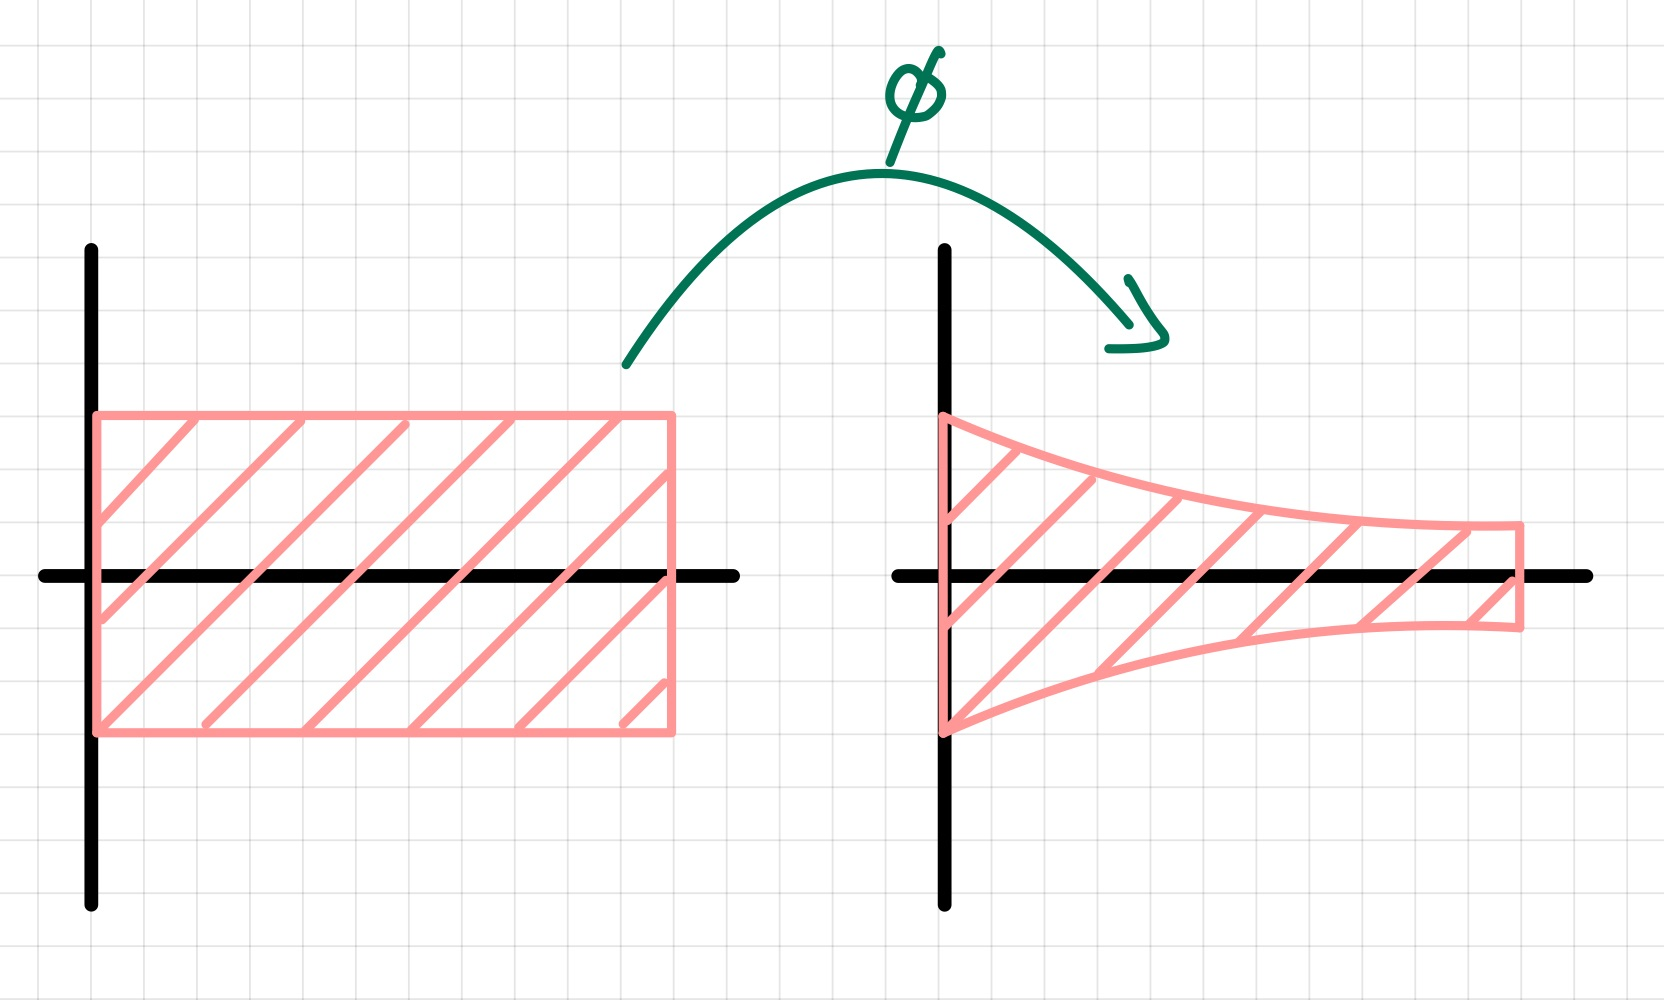
\includegraphics[width=\textwidth]{../\string_build/html/\string_images/trafo.jpg}
\caption{Visualisierung von Mengentransformationen.}\label{\detokenize{masstheorie/integrationstechnik:fig-trafo}}\end{figure}

\par
In \cref{masstheorie/masstheorie:rem:transinvariance} haben wir eine Matrix \(M\) und eine Menge \(M\) bereits die Identität
\begin{align*}
\lambda(MA) = |\det(M)| \, \lambda(A)
\end{align*}
\par
kennengelernt. Wir verllgemeinern diese Aussage nun, indem wir beliebige \(C^1\) Diffeomorphismen betrachten.
\begin{theorem}{}{masstheorie/integrationstechnik:thm:jacobitransformation}



\par
Seien \(U, V \subset \R^n\) offene Teilmengen und die Abbildung
\begin{align*}
\Phi \colon U \rightarrow V := \Phi(U)
\end{align*}
\par
sei ein \(C^1\) Diffeomorphismus, d.h., dass die Abbildung \(\Phi\) invertierbar ist, und dass sowohl \(\Phi\) als auch die Umkehrabbildung \(\Phi^{-1}\) stetig differenzierbar sind.
Sei außerdem \(f \colon V \rightarrow \R\) eine Lebesgue integrierbare Funktion.

\par
Dann gilt, dass die Verknüpfung \(f \circ \Phi \colon U \rightarrow \R\) auch Lebesgue integrierbar ist und es gilt die folgende Integrationsregel
\begin{align*}
\int_{\Phi(U)} f(y) \mu(\mathrm{d}y) = \int_U (f \circ \Phi)(x) \cdot |\det(D\Phi(x))|\mu(\mathrm{d}x).\end{align*}
\par
Hierbei nennt man \(\det(D\Phi(x))\) die \textbf{Jacobi Determinante}.
\end{theorem}

\begin{proof}
 Siehe z.B. \cite{Bog07} Theorem 3.7.1.
\end{proof}
\begin{remark}{}{masstheorie/integrationstechnik:remark-25}



\par
Für \(n=1\) ist diese Regel schon als Substitutionsregel bekannt.
\end{remark}
\begin{example}{}{masstheorie/integrationstechnik:example-26}



\par
ToDo
\end{example}


